\begin{chapterpage}{Foundations for inference}
  \chaptertitle{Foundations for inference}
  \label{foundationsForInference}
  \label{ch_foundations_for_inf}
  \label{ch_inference_foundations}
  \chaptersection{pointEstimates}
  \chaptersection{confidenceIntervals}
  \chaptersection{hypothesisTesting}
\end{chapterpage}
\renewcommand{\chapterfolder}{ch_foundations_for_inf}




\chapterintro{

Statistical inference is primarily concerned with
  understanding and quantifying the uncertainty of parameter estimates.
  While the equations and details change
  depending on the setting, the foundations for inference
  are the same throughout all of statistics.
  We start with a familiar topic:
  the idea of using a sample proportion to estimate a population proportion.
  Next, we create what's called a
  \emph{\hiddenterm{confidence interval}}, which is a range
  of values where the true population value is likely to lie.
  Finally, we introduce a \index{hypothesis test|textbf}%
  \emph{hypothesis testing framework},
  which allows us use data to formally evaluate claims about the
  population, such as whether a survey provides strong
  evidence that a candidate has the support of a majority
  of the voting population.}

%______________________________________________
\section[Estimating unknown parameters]{Estimating unknown parameters }
\label{pointEstimates}

\sectionintro{
\noindent%
Companies such as the Gallup and Pew Research frequently conduct
polls as a way to understand the state of public opinion
or knowledge on many topics, including politics,
scientific understanding, brand recognition, and more.  How well do these polls estimate the opinion or knowledge of the
broader population?  Why is a larger sample generally preferable to a smaller sample?  And what role does the concept of a sampling distribution, introduced in the previous chapter, play in answering these questions?


\subsection*{Learning objectives}
\begin{enumerate}
\item Explain the difference between probability and inference and identify when to use which one.

\item Understand the purpose and use of a point estimate.

\item Understand how to measure the variability/error in a point estimate.

\item Recognize the relationship between the standard error of a point estimate and the standard deviation of a sample statistic.

\item Understand how changing the sample size affects the variability/error in a point estimate.
\end{enumerate}
}


\D{\newpage}

%%
\subsection{Point estimates}
\index{point estimate|(}

With this chapter, we move from the world of probability to the world of inference.  Whereas \term{probability} involves using a known population value (parameter) to make a prediction about the likelihood of a particular sample value (statistic), \term{inference} involves using a calculated sample value (statistic) to estimate or better understand an unknown population value (parameter).  For both of these, the concept of the sampling distribution is fundamental.  

Suppose a poll suggested the US President's approval
rating is 45\%.
We would consider 45\% to be a
\term{point estimate}\index{estimate} of the approval
rating we might see if we collected responses from the
entire population.  This entire-population response proportion is
generally referred to as the \term{parameter}
of interest\index{parameter of interest},
and when the parameter is a proportion,
we denote it with the letter $p$. We typically estimate the parameter by collecting
information from a sample of the population;
we compute the observed proportion in the sample and we denote this sample proportion as $\hat{p}$.  Unless we collect responses from every individual in the sample,
$p$ remains unknown, and we use $\hat{p}$ as our point estimate for~$p$.

The difference we observe from the poll versus
the parameter is called the \term{error} in the estimate.  Generally, the error consists of two aspects:
sampling error and bias.

\termsub{Bias}{bias} describes a systematic tendency
to over- or under-estimate the true population value.
 For instance, if we took a political poll but our sample
  didn't include a roughly representative distribution of
  the political parties, the sample would likely skew
  in a particular direction and be biased.  Taking a truly random sample helps avoid bias.  However, as we saw in Chapter~\ref{ch_data_collection}, even with a random sample, various types of response bias can still be present.  For~example, if we were taking a student poll asking
about support for a new college stadium, we'd probably
get a biased estimate of the stadium's level of student
support by wording the question as,
\emph{Do you support your school by supporting funding
  for the new stadium?}
We try to minimize bias through thoughtful data
collection procedures, but bias can creep into our estimates without us even be aware.

  \termsub{Sampling error}{sampling error} is uncertainty in a point estimate that happens naturally from one sample to the next. Much of statistics, including much of this book, is focused on understanding and quantifying sampling error.  Remember though, that sampling error does not account for the possible effects of leading questions or other types of response bias.  When we measure sampling error, we are measuring the expected variability in a point estimate that arises from randomly sampling only a subset of the population.


\begin{examplewrap}
\begin{nexample}{
In Chapter~\ref{summarizingData}, we found the summary statistics for the number of characters in a set of 50 email data. These values are summarized below.

\begin{tabular}{l r }
$\bar{x}$ & 11,160 \\
median & 6,890 \\
$s_x$ & 13,130
\end{tabular}

Estimate the \term{population mean} based on the sample.}The best estimate for the population mean is the \term{sample mean}. That is,
$\bar{x} = 11,160$ is our best estimate for $\mu$.
\end{nexample}
\end{examplewrap}

\begin{exercisewrap}
\begin{nexercise}Using the email data, what quantity should we use as a point estimate for the population standard deviation $\sigma$?\footnotemark
\end{nexercise}
\end{exercisewrap}
\footnotetext{Again, intuitively we would use the sample standard deviation $s = 13,130$ as our best estimate for $\sigma$.}



%\Comment{add this discussion along with graphs for second edition?}
%\Cut{
%We will say that point estimate is \term{accurate} if the average of all of its possible values is the true population parameter. We will say that a point estimate is \term{precise} if it has low variability.
%
%Why do we want a point estimate to be both accurate and precise?
%}


\D{\newpage}

%%
\subsection{Understanding the variability of a point estimate}
\label{simulationForUnderstandingVariabilitySection}

\newcommand{\pewsolarpollsize}{1000}
\newcommand{\pewsolarparprop}{0.88}
\newcommand{\pewsolarparpropcomplement}{0.12}
\newcommand{\pewsolarparpercent}{88\%}
\newcommand{\pewsolarparpercentcomplement}{12\%}
\newcommand{\pewsolarpollprop}{0.887}
\newcommand{\pewsolarpollpropcomplement}{0.113}
\newcommand{\pewsolarpollpercent}{88.7\%}
\newcommand{\pewsolarpollpercentcomplement}{11.3\%}
\newcommand{\pewsolarpollcount}{887}
\newcommand{\pewsolarpollexpcount}{880}
\newcommand{\pewsolarpollcountcomplement}{113}
\newcommand{\pewsolarpollexpcountcomplement}{120}
\newcommand{\pewsolarpollse}{0.010}

Suppose the proportion of American adults who support
the expansion of solar energy is $p = \pewsolarparprop{}$,
which is our parameter of interest.\footnote{We haven't
  actually conducted a census to measure this value perfectly.
  However, a very large sample has suggested the actual
  level of support is about \pewsolarparpercent{}.}
If we were to take a poll of \pewsolarpollsize{} American adults
on this topic, the estimate would not be perfect,
but how close might we expect the sample proportion
in the poll would be to \pewsolarparpercent{}?
We want to understand, \emph{how does the
sample proportion $\hat{p}$ behave when the true population
proportion is \pewsolarparprop{}}.\footnote{Note:
  \pewsolarparpercent{} written as a proportion would be
  \pewsolarparprop{}.
  It is common to switch between proportion and percent.}
Let's find out!
We can simulate responses we would get from a simple
random sample of 1000 American adults,
which is only possible because we know the actual
support expanding solar energy to be \pewsolarparprop{}.  Here's how we might go about constructing such a simulation:
%simulate it:
\begin{enumerate}
\item There were about 250 million American adults in 2018.
    On 250 million pieces of paper, write ``support''
    on \pewsolarparpercent{} of them and ``not'' on
    the other \pewsolarparpercentcomplement{}.
\item Mix up the pieces of paper and pull out \pewsolarpollsize{}
    pieces to represent our sample of \pewsolarpollsize{}
    American adults.
\item Compute the fraction of the sample that say ``support''.
\end{enumerate}
Any volunteers to conduct this simulation? Probably not. While this physical simulation is totally impractical, we can simulate it thousands, even millions, of times using computer code.  We've written a short computer simulation and run it 10,000 times.  The results are show in 
Figure~\ref{solarPollSimulationCodeR}
in case you are curious what the computer code looks like.
In this simulation, the sample gave a point estimate of
$\hat{p}_1 = 0.894$. We~know the population proportion
for the simulation was $p = \pewsolarparprop{}$, so we know
the estimate had an error of
$0.894 - \pewsolarparprop{} = \text{+0.014}$.\D{\vspace{10mm}\\\ }


%\setlength\textwidth{\officialtextwidth-10mm}
\begin{figure}[h]
\texttt{\# 1.\ Create a set of 250 million entries,
where \pewsolarparpercent{} of them are "support" \\
\#\ \ \ \ and \pewsolarparpercentcomplement{} are "not". \\
pop\us{}size <- 250000000 \\
possible\_entries <- c(rep("support", \pewsolarparprop{} * pop\us{}size), rep("not", \pewsolarparpropcomplement{} * pop\us{}size))
\\[3mm]
\# 2.\ Sample \pewsolarpollsize{} entries without replacement. \\
sampled\_entries <- sample(possible\_entries, size = \pewsolarpollsize{}) \\[3mm]
\# 3.\ Compute p-hat:~count the number that are "support",
then divide by \\
\#\ \ \ \ the sample size. \\
sum(sampled\_entries == "support") / \pewsolarpollsize{}}
\caption{For those curious, this is code for
    a single $\hat{p}$ simulation using the
    statistical software called \R{}\index{R}.
    Each line that starts with \texttt{\#} is a
    \term{code comment},
    which is used to describe in regular language what the
    code is doing. We've provided software labs in \R{} at
    \oiRedirect{openintroorg_labs}{openintro.org/stat/labs}
    for anyone interested in learning more.}
\label{solarPollSimulationCodeR}
\end{figure}
% \setlength\textwidth{\officialtextwidth}

\D{\newpage}

One simulation isn't enough to get a great sense of the
distribution of estimates we might expect in the simulation,
so we should run more simulations.
In a second simulation,
we get $\hat{p}_2 = 0.885$, which has an error of~+0.005.
In another, $\hat{p}_3 = 0.878$ for an error of -0.002.
And in another,
an estimate of $\hat{p}_4 = 0.859$ with an error of -0.021.
With the help of a computer, we've run the simulation 10,000 times
and created a histogram of the results from all 10,000 simulations
in Figure~\ref{sampling_10k_prop_88p}. This
distribution of sample proportions is called a
\term{sampling distribution}.
We can characterize this sampling distribution as follows:
\begin{description}
\setlength{\itemsep}{0mm}
\item[Center.]
    The center of the distribution is
    $\mu_{\hat{p}} = \pewsolarparprop{}0$,
    which is the same as the parameter.
    Notice that the simulation mimicked a simple random sample
    of the population, which is a straightforward sampling
    strategy that helps avoid sampling bias.
%    That~is, we see that the sample proportion is an
%    \termsub{unbiased estimate}{unbiased}
%    of the population proportion.
\item[Spread.]
    The standard deviation of the distribution
    is $\sigma_{\hat{p}} = \pewsolarpollse{}$.
  
\item[Shape.]
    The distribution is symmetric and bell-shaped,
    and it \emph{resembles a normal distribution}.
\end{description}
These findings are encouraging!
When the population
proportion is $p = \pewsolarparprop{}$ and the sample size is
$n = \pewsolarpollsize{}$,
the sample proportion $\hat{p}$ tends to give
a pretty good estimate
of the population proportion.
We also have the interesting observation
that the histogram resembles a normal distribution.

\begin{figure}[h]
   \centering
   \Figure{0.85}{sampling_10k_prop_88p}
   \caption{A histogram of 10,000 sample proportions sampled from a population where the population
       proportion is \pewsolarparprop{} and the sample size is
       $n = \pewsolarpollsize{}$.}
   \label{sampling_10k_prop_88p}
\end{figure}

\begin{onebox}{Sampling distributions are
    never observed, but we keep them in mind}
  In real-world applications, we never actually observe the
  sampling distribution, yet it is useful to always think of
  a point estimate as coming from such a hypothetical
  distribution.
  \mbox{Understanding} the sampling distribution will help us
  characterize and make sense of the point estimates that we
  do observe.
\end{onebox}

\begin{examplewrap}
\begin{nexample}{If we used a much smaller sample size of $n = 50$,
would you guess that the standard error for $\hat{p}$ would be larger
or smaller than when we used $n = \pewsolarpollsize{}$?}
\label{smallerSampleWhatHappensToPropErrorExercise}
Intuitively, it seems like more data is better
than less data, and generally that is correct! The typical error
when $p = \pewsolarparprop{}$ and $n = 50$ would be larger
than the error we would expect when $n = \pewsolarpollsize{}$.
\end{nexample}
\end{examplewrap}

%\noindent
Example~\ref{smallerSampleWhatHappensToPropErrorExercise}
highlights an important property we will see again and again:
a bigger sample tends to provide a more precise point estimate
than a smaller sample.
Remember though, that this is only true for \emph{random} samples.
Additionally, a~bigger sample cannot correct for response bias or other types of bias that may be present.


\D{\newpage}

%%
\subsection{Introducing the standard error}

Point estimates only approximate the population parameter.  How can we quantify the expected variability in a point estimate $\hat{p}$? The discussion in Section~\ref{distributionphat} tells us how. The variability in the distribution of $\hat{p}$ is given by its standard deviation. If we know the population proportion, we can calculate the standard deviation of the point estimate $\hat{p}$.  In our simulation we knew $p$ was 0.88.  Thus we can calculate the standard deviation as 
\begin{align*}
SD_{\hat{p}}&=\sqrt{\frac{p(1-p)}{n}} = \sqrt{\frac{(.088)(1-0.88)}{n}}= 0.01
\end{align*}
If we now look at the sampling distribution, we see that the typical distance sample proportions are from the true value of 0.88 is about 0.01.

\begin{examplewrap}
\begin{nexample}{Consider a random sample of size 80 from a population.  We find that 15\% of the sample support a controversial new ballot measure.  How far is our estimate likely to be from the true percent that support the measure?}  We would like to calculate the standard deviation of $\hat{p}$, but we run into a serious problem: $p$ is \emph{unknown}. In fact, when doing inference, $p$ must be unknown, otherwise it is illogical to try to estimate it. We cannot calculate the $SD$, but we can estimate it using, you might have guessed, the sample proportion $\hat{p}$.
\end{nexample}
\end{examplewrap}
 
This estimate of the standard deviation is known as the \termsub{standard error}{standard error}, or $\pmb{SE}$ for short.
\begin{align*}
SE_{\hat{p}}&=\sqrt{\frac{\hat{p}(1-\hat{p})}{n}}
\end{align*}

\begin{examplewrap}
\begin{nexample}{Calculate and interpret the $SE$ of $\hat{p}$ for the previous example.}
\begin{align*}
SE_{\hat{p}}=\sqrt{\frac{\hat{p}(1-\hat{p})}{n}} =\sqrt{\frac{0.15(1-0.15)}{80}}=0.04
\end{align*}
The typical or expected error in our estimate is 4\%.
\end{nexample}
\end{examplewrap}

\begin{examplewrap}
\begin{nexample}{If we quadruple the sample size from 80 to 320, what will happen to the $SE$?}
\begin{align*}
SE_{\hat{p}}=\sqrt{\frac{\hat{p}(1-\hat{p})}{n}} =\sqrt{\frac{0.15(1-0.15)}{320}}=0.02
\end{align*}
The larger the sample size, the smaller our standard error. This is consistent with intuition: the more data we have, the more reliable an estimate will tend to be. However, quadrupling the sample size does not reduce the error by a factor of 4. Because of the square root, the effect is to reduce the error by a factor $\sqrt{4}$, or 2. 
\end{nexample}
\end{examplewrap}


\D{\newpage}

%%
\subsection{Basic properties of point estimates}

We achieved three goals in this section. First, we determined that point estimates from a sample may be used to estimate population parameters. We also determined that these point estimates are not exact: they vary from one sample to another. Lastly, we quantified the uncertainty of the sample proportion using what we  call the standard error. 

Remember that the standard error only measures sampling error.  It does not account for bias that results from leading questions or other types of response bias.

When our sampling method produces estimates in an unbiased way, the sampling distribution will be \emph{centered} on the true value and we call the method \term{accurate}.  When the sampling method  produces estimates that have \emph{low variability}, the sampling distribution will have a low standard error, and we call the method \term{precise}.

\begin{figure}[h]
   \centering
\oiRedirect{desmos-foursamplingdistributions}{
   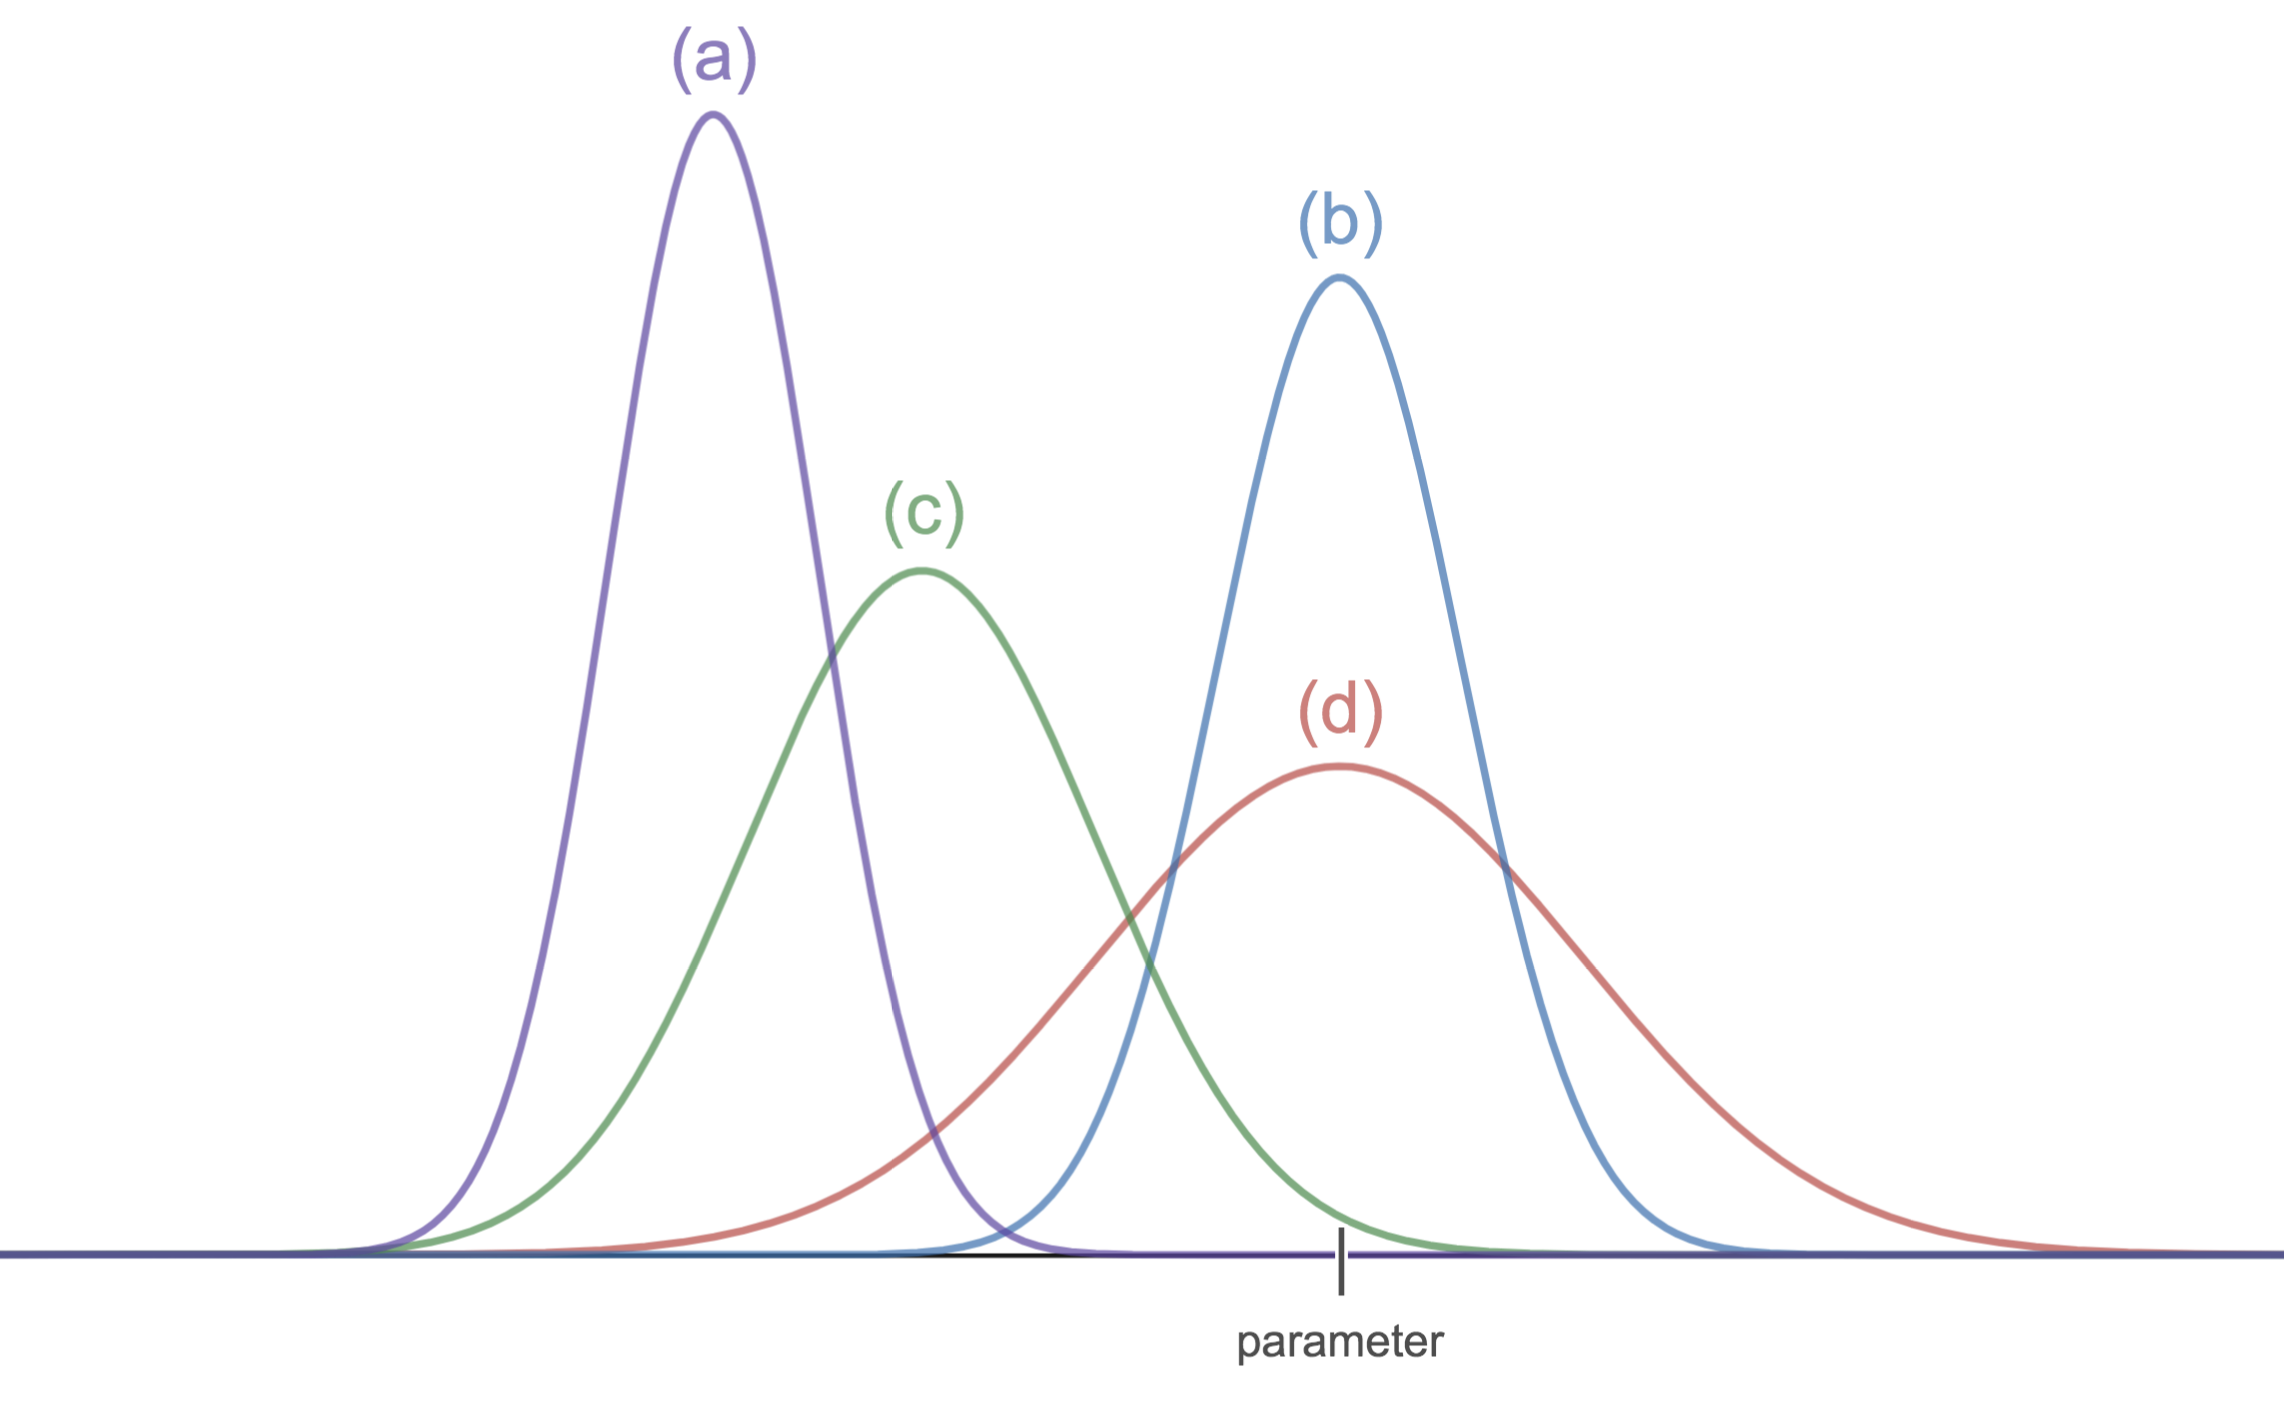
\includegraphics[width=0.59\textwidth]{ch_foundations_for_inf/figures/fourSamplingDistributions/fourSamplingDistributions}}
   \caption{Four sampling distributions shown, with parameter identified. Explore these distributions through a Desmos activity at \oiRedirect{openintro-ahss-desmos}{\small{openintro.org/ahss/desmos}}.}
   \label{fourSamplingDistributions}
\end{figure}

\begin{examplewrap}
\begin{nexample}
{Using Figure~\ref{fourSamplingDistributions}, which of the distributions were produced by methods that are biased?  That are accurate?  Order the distributions from most precise to least precise (that is, from lowest variability to highest variability).}
Distributions (b) and (d) are centered on the parameter (the true value), so those methods are accurate.  The methods that produced distributions (a) and (c) are biased, because those distributions are not centered on the parameter.  From most precise to least precise, we have (a), (b), (c), (d).
\end{nexample}
\end{examplewrap}

\begin{examplewrap}
\begin{nexample}
{Why do we want a point estimate to be both precise and accurate?} If the point estimate is precise, but highly biased, then we will consistently get a bad estimate.  On the other hand, if the point estimate is unbiased but not at all precise, then by random chance, we may get an estimate far from the true value.  

Remember, when taking a sample, we generally get only one chance.  It is the properties of the sampling distribution that tell us how much confidence we can have in the estimate. \end{nexample}
\end{examplewrap}

The strategy of using a sample statistic to estimate
a parameter is quite common, and it's a strategy that
we can apply to other statistics besides a proportion.
For instance, if we want to estimate the average salary
for graduates from a particular college, we could
survey a random sample of recent graduates;
in that example, we'd be using a sample mean $\bar{x}$
to estimate the population mean~$\mu$ for all graduates.
As another example, if we want to estimate the
difference in product prices for two websites,
we might take a random sample of products available
on both sites, check the prices on each,
and use then compute the average difference;
this strategy certainly wouldn't give us a perfect
measurement of the actual difference, but it would
give us a point estimate.

While this chapter emphases a single proportion
context, we'll encounter many different contexts
throughout this book where these methods will be
applied.
The principles and general ideas are the same,
even if the details change a little.



\D{\newpage}

%%
\subsection*{Section summary}
\begin{itemize}
\item In this section we laid the groundwork for our study of \term{inference}.  Inference involves using known sample values to estimate or better understand unknown population values.

\item  A sample statistic can serve as a \term{point estimate} for an unknown parameter.  For example, the sample mean is a point estimate for an unknown population mean, and the sample proportion is a point estimate for an unknown population proportion.

\item It is helpful to imagine a point estimate as being drawn from a particular sampling distribution.  

\item The \term{standard error} ($\textbf{SE}$) of a point estimate tells us the typical error or uncertainty associated with the point estimate.  It is also an estimate of the spread of the sampling distribution.  

\item A point estimate is \term{unbiased} (accurate) if the sampling distribution (i.e., the distribution of all possible outcomes of the point estimate from repeated samples from the same population) is \textit{centered} on the true population parameter.  

\item A point estimate has \term{lower variability} (more precise) when the \textit{standard deviation} of the sampling distribution is smaller. 

item In a random sample, increasing the sample size $n$ will make the standard error smaller.  This is consistent with the intuition that larger samples tend to be more reliable, all other things being equal.

\item In general, we want a point estimate to be unbiased and to have low variability.  Remember:  the terms unbiased (accurate) and low variability (precise) are properties of generic point estimates, which are variables that have a \emph{sampling distribution}.  These terms do not apply to individual values of a point estimate, which are \textit{numbers}.  

\end{itemize}


%%%%%%Section exercises
{\exercisesheader{}

% 1

\eoce{\qt{Identify the parameter, Part I\label{identify_parameter_1}} For each of the following situations, state 
whether the parameter of interest is a mean or a proportion. It may be helpful 
to examine whether individual responses are numerical or categorical.
\begin{parts}
\item In a survey, one hundred college students are asked how many hours per 
week they spend on the Internet.
\item In a survey, one hundred college students are asked: ``What percentage of 
the time you spend on the Internet is part of your course work?"
\item In a survey, one hundred college students are asked whether or not they 
cited information from Wikipedia in their papers.
\item In a survey, one hundred college students are asked what percentage of 
their total weekly spending is on alcoholic beverages.
\item In a sample of one hundred recent college graduates, it is found that 85 
percent expect to get a job within one year of their graduation date.
\end{parts}
}{}

% 2

\eoce{\qt{Identify the parameter, Part II\label{identify_parameter_2}} For each of the 
following situations, state whether the parameter of interest is a mean or a 
proportion. 
\begin{parts}
\item A poll shows that 64\% of Americans personally worry a great deal about 
federal spending and the budget deficit.
\item A survey reports that local TV news has shown a 17\% increase in revenue 
within a two year period while newspaper revenues decreased by 6.4\% during this 
time period.
\item In a survey, high school and college students are asked whether or not 
they use geolocation services on their smart phones.
\item In a survey, smart phone users are asked whether or not they use a web-based taxi service.
\item In a survey, smart phone users are asked how many times they used a web-based taxi service over the last year.
\end{parts}
}{}

% 3

\eoce{\qt{Quality control\label{comp_chips_quality_ctrl_prop}}
As part of a quality control process for computer chips,
an engineer at a factory randomly samples 212 chips
during a week of production to test the current rate of
chips with severe defects.
She finds that 27 of the chips are defective.
\begin{parts}
\item
    What population is under consideration in the data set?
\item
    What parameter is being estimated?
\item\label{comp_chips_quality_ctrl_prop_pt_est}%
    What is the point estimate for the parameter?
\item\label{comp_chips_quality_ctrl_prop_se_name}%
    What is the name of the statistic can we use to measure
    the uncertainty of the point estimate?
\item\label{comp_chips_quality_ctrl_prop_se_calc_w_pt_est}%
    Compute the value from
    part~(\ref{comp_chips_quality_ctrl_prop_se_name})
    for this context.
\item
    The historical rate of defects is 10\%.
    Should the engineer be surprised by the observed
    rate of defects during the current week?
\item
    Suppose the true population value was found to be 10\%.
    If we use this proportion to recompute the value in
    part~(\ref{comp_chips_quality_ctrl_prop_se_calc_w_pt_est})
    using $p = 0.1$ instead of $\hat{p}$,
    does the resulting value change much?
\end{parts}
}{}

% 4

\eoce{\qt{Unexpected expense\label{us_emergency_expense_prop}}
In a random sample 765 adults in the United States, 322 say
they could not cover a \$400 unexpected expense without borrowing
money or going into debt.
% Ref: https://www.federalreserve.gov/publications/files/2017-report-economic-well-being-us-households-201805.pdf
\begin{parts}
\item
    What population is under consideration in the data set?
\item
    What parameter is being estimated?
\item\label{us_emergency_expense_prop_pt_est}%
    What is the point estimate for the parameter?
\item\label{us_emergency_expense_prop_se_name}%
    What is the name of the statistic can we use to measure
    the uncertainty of the point estimate?
\item\label{us_emergency_expense_prop_se_calc_w_pt_est}%
    Compute the value from
    part~(\ref{us_emergency_expense_prop_se_name})
    for this context.
\item
    A cable news pundit thinks the value is actually 50\%.
    Should she be surprised by the data?
\item
    Suppose the true population value was found to be 40\%.
    If we use this proportion to recompute the value in
    part~(\ref{us_emergency_expense_prop_se_calc_w_pt_est})
    using $p = 0.4$ instead of $\hat{p}$,
    does the resulting value change much?
\end{parts}
}{}

\D{\newpage}

% 5

\eoce{\qt{Repeated water samples\label{repeated_water_samples_prop}}
A nonprofit wants to understand the fraction of households that
have elevated levels of lead in their drinking water.
They expect at least 5\% of homes will have elevated levels of
lead, but not more than about 30\%.
They randomly sample 800 homes and work with the owners to retrieve
water samples, and they compute the fraction of these homes
with elevated lead levels.
They repeat this 1,000 times and build a distribution
of sample proportions.
\begin{parts}
\item
    What is this distribution called?
\item
    Would you expect the shape of this distribution to be
    symmetric, right skewed, or left skewed?
    Explain your reasoning.
\item
    If the proportions are distributed around 8\%,
    what is the variability of the distribution?
\item
    What is the formal name of the value you computed in~(c)?
\item
    Suppose the researchers' budget is reduced, and they are only
    able to collect 250 observations per sample, but they can still
    collect 1,000 samples.
    They build a new distribution of sample proportions.
    How will the variability of this new distribution compare
    to the variability of the distribution when each sample
    contained 800 observations?
\end{parts}
}{}

% 6

\eoce{\qt{Repeated student samples\label{repeated_student_samples_prop}}
Of all freshman at a large college, 16\% made the dean's list
in the current year.
As part of a class project, students randomly sample 40 students
and check if those students made the list.
They repeat this 1,000 times and build a distribution
of sample proportions.
\begin{parts}
\item
    What is this distribution called?
\item
    Would you expect the shape of this distribution to be
    symmetric, right skewed, or left skewed?
    Explain your reasoning.
\item
    Calculate the variability of this distribution.
\item
    What is the formal name of the value you computed in~(c)?
\item
    Suppose the students decide to sample again,
    this time collecting 90 students per sample,
    and they again collect 1,000 samples.
    They build a new distribution of sample proportions.
    How will the variability of this new distribution compare
    to the variability of the distribution when each sample
    contained 40 observations?
\end{parts}
}{}
}



%_____________________________________
\section[Confidence intervals]{Confidence intervals }
\label{ConfidenceIntervals}
\label{confidenceIntervals}

\index{confidence interval|(}

\sectionintro{
\noindent%
The site \oiRedirect{textbook-fivethirtyeight}{fivethirtyeight.com} regularly forecasts support for each candidate in Congressional races, i.e. races in the
US House of Representatives and the US Senate.
In addition to point estimates, they report confidence intervals.\footnote{See: \oiRedirect{textbook-538-2018-midterm}{\url{https://projects.fivethirtyeight.com/2018-midterm-election-forecast/senate}}}
What are confidence intervals, and how do we interpret them?  


%%
\subsection*{Learning objectives}
\begin{enumerate}
\item Explain the purpose and use of confidence intervals.

\item Construct 95\% confidence intervals assuming the point estimate follows a normal distribution.

\item Calculate the critical value for a C\% confidence interval when the point estimate follows a normal distribution.

\item Describe how sample size and confidence level affect the width of a confidence interval.

\item Interpret a confidence interval and the confidence level in context.

\item Draw conclusions with a specified confidence level about the values of unknown parameters.  

\item Calculate and interpret the margin of error for a C\% confidence interval.  Distinguish between margin of error and standard error.
\end{enumerate}
}


%%
\subsection{Capturing the population parameter}

A point estimate provides a single plausible value for a parameter. However, a point estimate isn't perfect and will have some \emph{standard error} associated with it. When estimating a parameter,
it is better practice to provide a plausible
\emph{range of values} instead of supplying just the point
estimate.

A plausible range of values for the population parameter is called a \term{confidence interval}. Using only a point estimate is like fishing in a murky lake with a spear, and using a confidence interval is like fishing with a net. We can throw a spear where we saw a fish, but we will probably miss. On the other hand, if we toss a net in that area, we have a good chance of catching the fish.

If we report a point estimate, we probably will not hit the exact population parameter. On the other hand, if we report a range of plausible values -- a confidence interval -- we have a good shot at capturing the parameter.


\D{\newpage}

%%
\subsection{Constructing a 95\% confidence interval}

A point estimate is our best guess for the value of the parameter, so it makes sense to build the confidence interval around that value. The standard error is a measure of the uncertainty associated with the point estimate.  

\begin{examplewrap}
\begin{nexample}{How many standard errors should we extend above and below the point estimate if we want to be 95\% confident of capturing the true value?  }
First, we observe that the area under the standard normal curve between -1.96 and 1.96 is 95\%.  When conditions for a normal model are met, the point estimate we observe will be within 1.96 standard deviations of the true value about 95\% of the time.  Thus, if we want to be 95\% confident of capturing the true value, we should go 1.96 standard errors on either side of the point estimate.
\end{nexample}
\end{examplewrap}

\begin{onebox}{Constructing a 95\% confidence interval using a normal model}
When the sampling distribution of a point estimate can reasonably be modeled as normal, a 95\% confidence interval for the unknown parameter can be constructed as: \vspace{-2mm}
\begin{align}
\text{point estimate}\ \pm\ 1.96 \times SE\text{ of estimate}\vspace{-2mm}
\label{95PercentConfidenceIntervalFormula}
\end{align}
We can be \textbf{95\% confident} that this interval captures the true value.\end{onebox}

In the next chapters we will determine when we can apply a normal model to a point estimate. For now, we will assume that a normal model is reasonable. 

\begin{examplewrap}
\begin{nexample}{The point estimate from the smoking example was 15\%. The standard error for this point estimate was calculated to be $SE = 0.04$. Assuming that conditions for a normal model are met, construct and interpret a 95\% confidence interval.  }
\begin{align*}
\text{point estimate}\ &\pm \ 1.96\times SE \text{ of estimate} \\
0.15\  &\pm \ 1.96\times 0.04\\
(0.071&6\text{, } 0.2284)
\end{align*}
We are 95\% confident that the true percent of smokers in this population is between 7.16\% and 22.84\%.
\end{nexample}
\end{examplewrap}

\begin{examplewrap}
\begin{nexample}{Based on the confidence interval above, is there evidence that a smaller proportion smoke in this county than in the state as a whole? The proportion that smoke in the state is known to be 0.20.}While the point estimate of 0.15 is lower than 0.20, this deviation is likely due to random chance. Because the confidence interval \emph{includes} the value 0.20, 0.20 is a reasonable value for the proportion of smokers in the county. Therefore, based on this confidence interval, we do not have evidence that a smaller proportion smoke in the county than in the state.
\end{nexample}
\end{examplewrap}

We can be 95\% confident that a 95\% confidence interval captures the true population parameter. However, confidence intervals are imperfect. About 1-in-20 (5\%) properly constructed 95\% confidence intervals will fail to capture the parameter of interest. Figure~\ref{95PercentConfidenceInterval} shows 25 confidence intervals for a proportion that were constructed from simulations where the true proportion was $p = 0.3$. However, 1 of these 25 confidence intervals happened not to include the true value.

\begin{figure}[h]
\centering
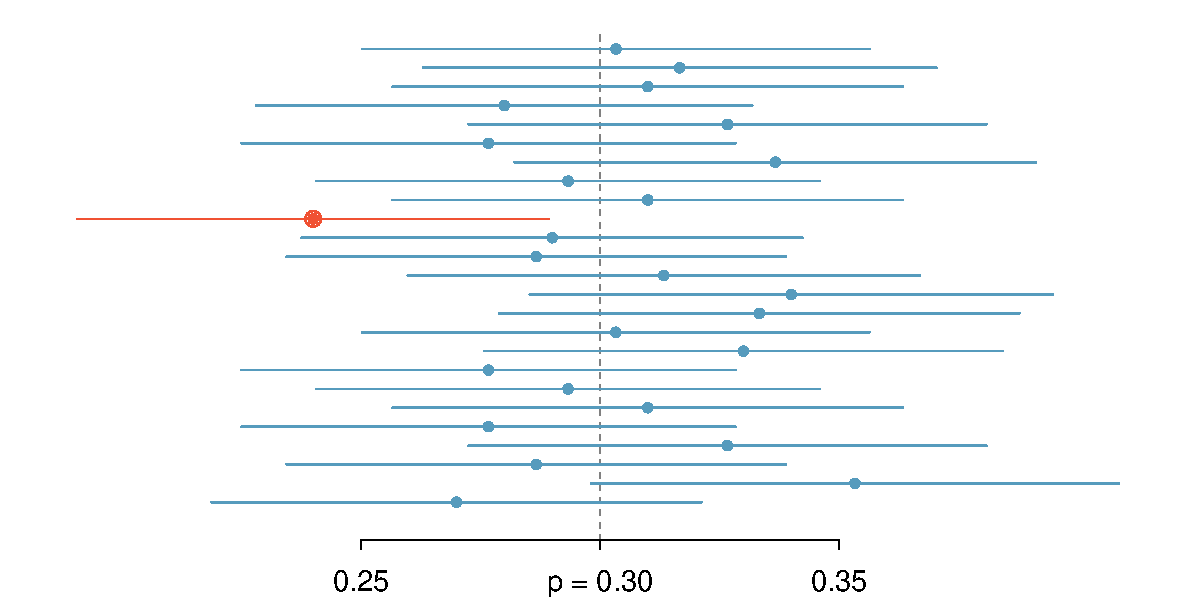
\includegraphics[width=0.9\textwidth]{ch_foundations_for_inf/figures/95PercentConfidenceInterval/95PercentConfidenceInterval}
\caption{Twenty-five samples of size $n=300$ were simulated when $p = 0.30$. For each sample, a confidence interval was created to try to capture the true proportion $p$. However,~1~of these~25 intervals did not capture $p = 0.30$.}
\label{95PercentConfidenceInterval}
\end{figure}

\begin{exercisewrap}
\begin{nexercise}
In Figure~\ref{95PercentConfidenceInterval}, one interval does not capture the true proportion, $p = 0.3$. Does this imply that there was a problem with the simulations?\footnotemark
\end{nexercise}
\end{exercisewrap}
\footnotetext{No. Just as some observations occur more than 1.96 standard deviations from the mean, some point estimates will be more than 1.96 standard errors from the parameter. A confidence interval only provides a plausible range of values for a parameter. While we might say other values are implausible based on the data, this does not mean they are impossible.}

%%
\subsection{Changing the confidence level}
\label{changingTheConfidenceLevelSection}

\index{confidence level|(}

Suppose we want to construct a confidence interval with a confidence level somewhat greater than 95\%: perhaps we would like a confidence level of 99\%. 

\begin{examplewrap}
\begin{nexample}{Other things being equal, would a 99\% confidence interval be wider or narrower than a 95\% confidence interval?}Using a previous analogy: if we want to be more confident that we will catch a fish, we should use a wider net, not a smaller one. To be 99\% confidence of capturing the true value, we must use a wider interval. On the other hand, if we want an interval with lower confidence, such as 90\%, we would use a narrower interval.
\end{nexample}
\end{examplewrap}

The 95\% confidence interval structure provides guidance in how to make intervals with new confidence levels. Below is a general 95\% confidence interval for a point estimate that comes from a nearly normal distribution:
\begin{eqnarray}
\text{point estimate}\ \pm\ 1.96\times SE \text{ of estimate}
\end{eqnarray}
There are three components to this interval: the point estimate, ``1.96'', and the standard error. The choice of $1.96\times SE$ was based on capturing 95\% of the distribution since the estimate is within 1.96 standard deviations of the true value about 95\% of the time. The choice of 1.96 corresponds to a 95\% confidence level. 

\D{\newpage}

\begin{exercisewrap}
\begin{nexercise} \label{leadInForMakingA99PercentCIExercise}
If $X$ is a normally distributed random variable, how often will $X$ be within 2.58 standard deviations of the mean?\footnotemark
\end{nexercise}
\end{exercisewrap}
\footnotetext{This is equivalent to asking how often the Z-score will be larger than -2.58 but less than 2.58. (For a picture, see Figure~\ref{choosingZForCI}.) There is $\approx$ 0.99 probability that the unobserved random variable $X$ will be within 2.58 standard deviations of the mean.}


\begin{figure}[ht]
\centering
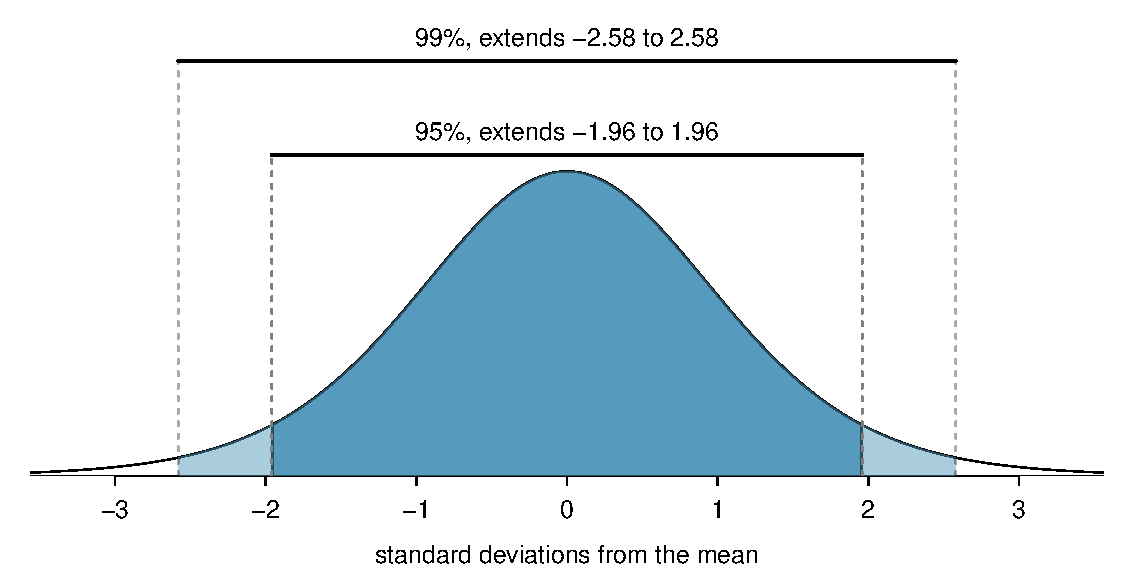
\includegraphics[width=\textwidth]{ch_foundations_for_inf/figures/choosingZForCI/choosingZForCI}
\caption{The area between -$z^{\star}$ and $z^{\star}$ increases as $|z^{\star}|$ becomes larger. If the confidence level is 99\%, we choose $z^{\star}$ such that 99\% of the normal curve is between -$z^{\star}$ and $z^{\star}$, which corresponds to 0.5\% in the lower tail and 0.5\% in the upper tail: $z^{\star}=2.58$.}
\label{choosingZForCI}
\index{confidence level|)}
\end{figure}


To create a 99\% confidence interval, change 1.96 in the 95\% confidence interval formula to be $2.58$. Guided Practice~\ref{leadInForMakingA99PercentCIExercise} highlights that 99\% of the time a normal random variable will be within 2.58 standard deviations of its mean. Thus, the formula for a 99\% confidence interval is
\begin{eqnarray}
\text{point estimate}\ \pm\ 2.58\times SE \text{ of estimate}
\label{99PercCIForMean}
\label{99PercCIForNormalPointEstimate}
\end{eqnarray}
%\Comment{I don't know where the equation number above gets referenced. Might drop the equation number.}
Figure~\ref{choosingZForCI} provides a picture of how to identify $z^{\star}$ based on a confidence level. 

The \emph{number} of standard errors we go above and below the point estimate is called the \term{critical value}.  When the critical value is determined based on a normal model, we call the critical value $z^{\star}$. 

\begin{onebox}{Confidence interval for any confidence level}
If the point estimate follows a normal model with standard error $SE$, then a confidence interval for the population parameter is
\begin{eqnarray*}
\text{point estimate}\ \pm\ z^{\star} \times SE \text{ of estimate}
\end{eqnarray*}
where $z^{\star}$ depends on the confidence level selected.\end{onebox}

Finding the value of $z^{\star}$ that corresponds to a particular confidence level is most easily accomplished by using a new table, called the $t$-table. For now, what is noteworthy about this table is that the bottom row corresponds to confidence levels. The numbers inside the table are the critical values, but which row should we use? Later in this book, we will see that a $t$-curve with infinite degrees of freedom corresponds to the normal curve. For this reason, when finding $z^{\star}$, we use the $t$-table at row $\infty$.

\D{\newpage}

\begin{figure}[hht]
\centering
\begin{tabular}{r | rrr rr}
one tail & \hspace{1.5mm}  0.100 & \hspace{1.5mm} 0.050 & \hspace{1.5mm} 0.025 & \hspace{1.5mm} 0.010 & \hspace{1.5mm} 0.005  \\
\hline
{$df$} \hfill 1  &  {\normalsize  3.078} & {\normalsize  6.314} & {\normalsize 12.71} & {\normalsize 31.82} & {\normalsize 63.66}  \\ 
2  &  {\normalsize  1.886} & {\normalsize  2.920} & {\normalsize  4.303} & {\normalsize  6.965} & {\normalsize  9.925}  \\ 
3  &  {\normalsize  1.638} & {\normalsize  2.353} & {\normalsize  3.182} & {\normalsize  4.541} & {\normalsize  5.841}  \\ 
$\vdots$ & $\vdots$ &$\vdots$ &$\vdots$ &$\vdots$ & \\
1000  &  {\normalsize  1.282} & {\normalsize  1.646} & {\normalsize  1.962} & {\normalsize  2.330} & {\normalsize  2.581}  \\ 
$\infty$   &  {\normalsize  1.282} & {\normalsize  1.645} & {\normalsize  1.960} & {\normalsize  2.326} & {\normalsize  2.576}   \\
\hline
Confidence level C  &  {\normalsize  80\%} & {\normalsize 90\%} & {\normalsize 95\%} & {\normalsize  98\%} & {\normalsize  99\%}  \\
\hline
\end{tabular}
\caption{An abbreviated look at the $t$-table. The columns correspond to confidence levels. Row $\infty$ corresponds to the normal curve.}
\label{tTableSample}
\end{figure}


\begin{onebox}{Finding \pmb{$\MakeLowercase{z}^{\star}$ }for a particular confidence level}
We select $z^{\star}$ so that the area between -$z^{\star}$ and $z^{\star}$ in the normal model corresponds to the confidence level. Use a calculator or use the $t$-table at row $\infty$ to find the critical value $z^{\star}$.\end{onebox}

\begin{exercisewrap}
\begin{nexercise} \label{find90CIForRun10AgeExercise}
Find the appropriate $z^{\star}$ value for an 80\% confidence interval.\footnotemark
\end{nexercise}
\end{exercisewrap}
\footnotetext{Using row $\infty$ on the $t$-table, we see that the value that corresponds to an 80\% confidence level is 1.282.  Therefore, we should use 1.282 as the $z^{\star}$ value.  }

The normal approximation is crucial to the precision of these confidence intervals. The next two chapters provide detailed discussions about when a normal model can safely be applied to a variety of situations. When a normal model is not a good fit, we will use alternate distributions that better characterize the sampling distribution.

%%
\subsection{Margin of error}

The confidence intervals we have encountered thus far have taken the form
\begin{align*}
\text{point estimate} \ \pm \ z^*\times SE \text{ of estimate}
\end{align*}
Confidence intervals are also often reported as 
\begin{align*}
\text{point estimate} \ \pm \ \text{margin of error}
\end{align*}
For example, instead of reporting an interval as $0.09 \ \pm  \ 1.645\times 0.028$ or $(0.044, 0.136)$, it could be reported as $0.09 \ \pm \  0.046$.

The \term{margin of error} is the distance between the point estimate and the lower or upper bound of a confidence interval.  It is half of the total width of the interval.

\begin{onebox}{Margin of error}\label{marginOfErrorTermBox}
When the point estimate follows a normal distribution, 
$$ \text{margin of error} = z^{\star}\times SE \text{ of estimate}.$$
\end{onebox}

\D{\newpage}

\begin{examplewrap}
\begin{nexample}{All other things being equal, will the margin of error be bigger for a 68\% confidence interval or a 95\% confidence interval?}
A 95\% confidence interval is wider than a 68\% confidence interval and has a larger $z^{\star}$ value, so the 95\% confidence interval will have a larger margin of error.
\end{nexample}
\end{examplewrap}

\begin{exercisewrap}
\begin{nexercise}What is the margin of error for the confidence interval: (0.035, 0.145)?\footnotemark
\end{nexercise}
\end{exercisewrap}
\footnotetext{The margin of error is \emph{half} of the total width of the interval. The margin of error for this interval is $\frac{0.145 - 0.035}{2}=0.055$.}

%%
\subsection{Interpreting confidence intervals}
\label{interpretingCIs}

\index{confidence interval!interpretation|(}

A careful eye might have observed the somewhat awkward language used to describe confidence intervals. Correct interpretation:
\begin{quote}
We are C\% confident that the population parameter is between \underline{\ \ \ \ \ } and \underline{\ \ \ \ \ }.
\end{quote}
\emph{Incorrect} language might try to describe the confidence interval as capturing the population parameter with a certain probability.\footnote{To see that this interpretation is incorrect, imagine taking two random samples and constructing two 95\% confidence intervals for an unknown proportion. If these intervals are disjoint, can we say that there is a 95\%+95\%=190\% chance that the first or the second interval captures the true value?} Applying the language of probability to a fixed interval or to a fixed parameter is one of the most common errors.  

As we saw in Figure~\ref{95PercentConfidenceInterval}, the 95\% confidence interval \emph{method} has a 95\% probability of producing an interval that will capture the population parameter. A correct interpretation of the confidence \emph{level} is that such intervals will capture the population parameter that percent of the time (assuming conditions are met and the probability model is true). However, each individual interval either does or does not capture the population parameter. A correct interpretation of an individual confidence interval cannot involve the vocabulary of probability.

Another especially important consideration of confidence intervals is that they \emph{only try to capture the population parameter}. Our intervals say nothing about the confidence of capturing individual observations, a proportion of the observations, or point estimates. Confidence intervals only attempt to capture population parameters.

\index{confidence interval!interpretation|)}
\index{confidence interval|)}


%%
\subsection{Confidence interval procedures: a five step process}

Use a confidence interval to \emph{estimate} a parameter with a particular \emph{confidence level}, C.

\begin{onebox}{(AP exam tip) When carrying out a confidence intervaL procedure, follow these five steps:}
\begin{itemize}
\setlength{\itemsep}{0mm}
\item \inferencestep{Identify}  Identify the parameter and the confidence level.
\item  \inferencestep{Choose}  Choose the appropriate interval procedure and identify it by name.
\item  \inferencestep{Check}  Check that the conditions for the interval procedure are met. 
\item \inferencestep{Calculate} Calculate the confidence interval and record it in interval form.  
\begin{align*}
\text{CI:  point estimate}\ \pm\  \text{critical value}\times SE \text{ of estimate}
\end{align*}
\item \inferencestep{Conclude} Interpret the interval and, if applicable, draw a conclusion based on whether the interval is entirely above, is entirely below, or contains the value of interest.
\end{itemize}\end{onebox}

\index{confidence interval|)}


\D{\newpage}

%%
\subsection*{Section summary}
\begin{itemize}
\item A point estimate is not perfect; there is almost always some error in the estimate. It is often useful to supply a plausible \textit{range of values} for the parameter, which we call a \term{confidence interval}.  

\item A confidence interval is centered on the point estimate and extends a certain number of standard errors on either side of the estimate, depending upon how \textit{confident} one wants to be.  For a fixed sample size, to be more confident of capturing the true value requires a wider interval.


\item When the sampling distribution of a point estimate can reasonably be modeled as
\emph{normal}, such as with a \term{sample proportion}, then the following are true:\vspace{-1mm}
\begin{itemize}
\item A 68\% confidence interval is given by:  point estimate\ $\pm\ SE$ of estimate.
\\We can be 68\% confident this interval captures the true value.
\item A 95\% confidence interval is given by:   point estimate\ $\pm\ 1.96 \times SE$ of estimate.
\\We can be 95\% confident this interval captures the true value.
\item A C\% confidence interval is given by:   point estimate\ $\pm\ z^{\star} \times SE$ of estimate.  
\\We can be C\% confident this interval captures the true value.
\end{itemize}

\item For a C\% confidence interval described above, we select $z^{\star}$ such that the area between -$z^{\star}$ and $z^{\star}$ under the standard normal curve is C\%. Use the $t$-table at row $\infty$ to find the critical value $z^{\star}$.\footnote{We explain the relationship between $z$ and $t$ in the next chapter.}

\item After interpreting the interval, we can usually draw a conclusion, with C\% confidence, about whether a given value X is a reasonable value for the population parameter.  When drawing a conclusion based on a confidence interval, there are three  possibilities.  

\begin{itemize}\vspace{-1mm}
\setlength{\itemsep}{0mm}
\item We \emph{have evidence} that the true [parameter]:
\begin{itemize}\vspace{-1mm}
\setlength{\itemsep}{0mm}
\item[]  ...is greater than X, because the entire interval is \emph{above} X.
\item[] ...is less than X, because the entire interval is \emph{below} X.
\end{itemize}
\item We \emph{do not have evidence} that the true [parameter] is not  X, because X is \emph{in} the interval.
\end{itemize}

\item AP exam tip:  A full confidence interval procedure includes the following steps. \vspace{-1mm}
\begin{enumerate}
\setlength{\itemsep}{0mm}
\item \inferencestep{Identify}  Identify the parameter and the confidence level.
\item  \inferencestep{Choose}  Choose the appropriate interval procedure and identify it by name.
\item  \inferencestep{Check}  Check that the conditions for the interval procedure are met. 
\item \inferencestep{Calculate} Calculate the confidence interval and record it in interval form.  
\begin{align*}
\text{CI:  point estimate}\ \pm\  \text{critical value}\times SE \text{ of estimate}
\end{align*}
\item \inferencestep{Conclude} Interpret the interval and, if applicable, draw a conclusion based on whether the interval is entirely above, is entirely below, or contains the value of interest.
\item[]
\end{enumerate}
\end{itemize}
Interpreting \termsub{confidence intervals}{confidence interval} and \termsub{confidence levels}{confidence level}
\begin{itemize}
\item 68\% and 95\% are examples of \termsub{confidence levels}{confidence level}.  The confidence level tells us the \emph{capture rate} with repeated sampling.  For example, a correct interpretation of a 95\% confidence level is that if many samples of the same size were taken from the population, about 95\% of the resulting confidence intervals would capture the true population parameter (assuming the conditions are met and the probability model is true).  Note that this is a \emph{relative frequency interpretation}.  

\item We cannot use the language of probability to interpret an \emph{individual} confidence interval, once it has been calculated.  The confidence level tells us what percent of the intervals will capture the population parameter, not the probability that a calculated interval captures the population parameter.  Each calculated interval either does or does not capture the population parameter.  
\end{itemize}


\D{\newpage\noindent%
}\termsub{Margin of error}{margin of error}
\noindent\begin{itemize}
\item Confidence intervals are often reported as: point estimate $\pm$ margin of error.  The \term{margin of error} ($ME$) $=\text{critical value} \times SE\ \text{of estimate}$, and it tells us, with a particular confidence, how much we expect our point estimate to deviate from the true population value due to chance.  

\item The margin of error depends on the \emph{confidence level}; the standard error does not.  Other things being constant, a higher confidence level leads to a larger margin of error.  

\item For a fixed confidence level, increasing the sample size decreases the margin of error.  This assumes a random sample.

\item The margin of error formula only applies if a sample is random.  Moreover, the margin of error measures only \emph{sampling error}; it does not account for additional error introduced by response bias and non-response bias.  Even with a perfectly random sample, the actual error in a poll is likely higher than the reported margin of error.\footnote{\oiRedirect{textbook-nytimes_moe_think_7_instead}{nytimes.com/2016/10/06/upshot/when-you-hear-the-margin-of-error-is-plus-or-minus-3-percent-think-7-instead.html}}

\end{itemize}


%%%%%%Section exercises
{\exercisesheader{}

% 7 - chronic_illness_intro

\eoce{\qt{Chronic illness, Part I\label{chronic_illness_intro}} 
In 2013, the Pew Research Foundation reported that ``45\% of U.S. adults report 
that they live with one or more chronic conditions''.
\footfullcite{data:pewdiagnosis:2013} However, this value was based on a sample, 
so it may not be a perfect estimate for the population parameter of interest on 
its own. The study reported a standard error of about 1.2\%, and a normal model 
may reasonably be used in this setting. Create a 95\% confidence interval for 
the proportion of U.S. adults who live with one or more chronic conditions. Also 
interpret the confidence interval in the context of the study.
}{}

% 8 - twitter_users_intro

\eoce{\qt{Twitter users and news, Part I\label{twitter_users_intro}} 
A poll conducted in 2013 found that 52\% of U.S. adult Twitter users 
get at least some news on Twitter.\footfullcite{data:pewtwitternews:2013}. 
The standard error for this estimate was 2.4\%, and a normal distribution 
may be used to model the sample proportion. Construct a 99\% confidence 
interval for the fraction of U.S. adult Twitter users who get some 
news on Twitter, and interpret the confidence interval in context.
}{}

% 9 - chronic_illness_tf

\eoce{\qt{Chronic illness, Part II\label{chronic_illness_tf}} In 2013, the Pew Research Foundation reported that 
``45\% of U.S. adults report that they live with one or more chronic 
conditions'', and the standard error for this estimate is 1.2\%. Identify each 
of the following statements as true or false. Provide an explanation to justify 
each of your answers.
\begin{parts}
\item We can say with certainty that the confidence interval from 
Exercise~\ref{chronic_illness_intro} contains the true percentage of U.S. adults who 
suffer from a chronic illness.
\item If we repeated this study 1,000 times and constructed a 95\% confidence 
interval for each study, then approximately 950 of those confidence intervals 
would contain the true fraction of U.S. adults who suffer from chronic illnesses.
\item The poll provides statistically significant evidence (at the 
$\alpha = 0.05$ level) that the percentage of U.S. adults who suffer from 
chronic illnesses is below 50\%.
\item Since the standard error is 1.2\%, only 1.2\% of people in the study 
communicated uncertainty about their answer.
\end{parts}
}{}

% 10 - twitter_users_tf

\eoce{\qt{Twitter users and news, Part II\label{twitter_users_tf}} A poll conducted in 2013 found that 52\% of 
U.S. adult Twitter users get at least some news on Twitter, and the standard 
error for this estimate was 2.4\%. Identify each of the following statements as 
true or false. Provide an explanation to justify each of your answers.
\begin{parts}
\item The data provide statistically significant evidence that more than half of 
U.S. adult Twitter users get some news through Twitter. Use a significance level 
of $\alpha = 0.01$.
\item Since the standard error is 2.4\%, we can conclude that 97.6\% of all U.S. 
adult Twitter users were included in the study.
\item If we want to reduce the standard error of the estimate, we should collect 
less data.
\item If we construct a 90\% confidence interval for the percentage of U.S. 
adults Twitter users who get some news through Twitter, this confidence interval 
will be wider than a corresponding 99\% confidence interval.
\end{parts}
}{}

% 11 - er_wait_intro_prop_ok

\eoce{\qt{Waiting at an ER, Part I\label{er_wait_intro_prop_ok}} A hospital administrator 
hoping to improve wait times decides to estimate the average emergency 
room waiting time at her hospital. She collects a simple random sample 
of 64 patients and determines the time (in minutes) between when they 
checked in to the ER until they were first seen by a doctor. A 95\% 
confidence interval based on this sample is (128 minutes, 147 minutes), 
which is based on the normal model for the mean. Determine whether the 
following statements are true or false, and explain your reasoning.
\begin{parts}
\item We are 95\% confident that the average waiting time of these 64 emergency 
room patients is between 128 and 147 minutes.
\item We are 95\% confident that the average waiting time of all patients at 
this hospital's emergency room is between 128 and 147 minutes.
\item 95\% of random samples have a sample mean between 128 and 147 minutes.
\item A 99\% confidence interval would be narrower than the 95\% confidence 
interval since we need to be more sure of our estimate.
\item The margin of error is 9.5 and the sample mean is 137.5.
\item In order to decrease the margin of error of a 95\% confidence interval to 
half of what it is now, we would need to double the sample size.
\end{parts}
}{}

% 12 - mental_health

\eoce{\qt{Mental health\label{mental_health}}
The General Social Survey asked the question:
``For how many days during the past 30 days was your 
mental health, which includes stress, depression,
and problems with emotions, not good?"
Based on responses from 1,151 US residents,
the survey reported a 95\% confidence interval of
3.40 to 4.24 days in 2010.
\begin{parts}
\item
    Interpret this interval in context of the data.
\item
    What does ``95\% confident" mean? Explain in the
    context of the application.
\item
    Suppose the researchers think a 99\% confidence level
    would be more appropriate for this interval.
    Will this new interval be smaller or wider than the
    95\% confidence interval?
\item
    If a new survey were to be done with 500 Americans,
    do you think the standard error of the estimate be
    larger, smaller, or about the same.
\end{parts}
}{}
}

%_________________________________
\section[Introducing hypothesis testing]{Introducing hypothesis testing }
\label{hypothesisTesting}
\index{hypothesis testing|(}

\sectionintro{
\noindent%
In an experiment, one treatment reduces cholesterol by 10\% while another treatment reduces it by 17\%.  Is this strong enough evidence that the second treatment is more effective?
In this section, we will set up a framework for answering questions such as this and will look at the different types of decision errors that researcher can make when drawing conclusions based on data.


%%
\subsection*{Learning objectives}

\begin{enumerate}
\item Explain the logic of hypothesis testing, including setting up hypotheses and drawing a conclusion based on the set significance level and the calculated p-value.

\item Set up the null and alternative hypothesis in words and in terms of population parameters.


\item Interpret a p-value in context and recognize how the calculation of the p-value depends upon the direction of the alternative hypothesis. 

\item Define and interpret the concept statistically significant.

\item Interpret Type~I, Type~II Error, and power in the context of hypothesis testing.

\end{enumerate}
}



%%
\subsection{Case study: medical consultant}

\index{data!medical consultant|(}
People providing an organ for donation sometimes seek the help of a special medical consultant. These consultants assist the patient in all aspects of the surgery, with the goal of reducing the possibility of complications during the medical procedure and recovery. Patients might choose a consultant based in part on the historical complication rate of the consultant's clients.

One consultant tried to attract patients by noting the overall complication rate for liver donor surgeries in the US is about 10\%, but her clients have had only 9 complications in the 142 liver donor surgeries she has facilitated. She claims this is strong evidence that her work meaningfully contributes to reducing complications (and therefore she should be~hired!).

\begin{examplewrap}\begin{nexample}{We will let $p$ represent the true complication rate for liver donors working with this consultant. Calculate the best estimate for $p$ using the data.  Label the point estimate as $\hat{p}$.}
The sample proportion for the complication rate is 9~complications divided by the 142~surgeries the consultant has worked on: $\hat{p} = 9 / 142 = 0.063$.
\end{nexample}\end{examplewrap}

\begin{examplewrap}\begin{nexample}{Is it possible to prove that the consultant's work reduces complications?}
No. The claim implies that there is a causal connection, but the data are observational. For example, maybe patients who can afford a medical consultant can afford better medical care, which can also lead to a lower complication rate.
\end{nexample}\end{examplewrap}

\begin{examplewrap}\begin{nexample}{While it is not possible to assess the causal claim, it is still possible to ask whether the low complication rate of $\hat{p} = 0.063$ provides evidence that the consultant's true complication rate is different than the US complication rate. Why might we be tempted to immediately conclude that the consultant's true complication rate is different than the US complication rate? Can we draw this conclusion?}
Her sample complication rate is $\hat{p} = 0.063$, which is 0.037 lower than the US complication rate of 10\%. However, we cannot yet be sure if the observed difference represents a real difference or is just the result of random variation. We wouldn't expect the sample proportion to be \emph{exactly} 0.10, even if the truth was that her real complication rate was 0.10.
\end{nexample}\end{examplewrap}


%%
\subsection{Setting up the null and alternate hypothesis}

We can set up two competing hypotheses about the consultant's true complication rate. The first is call the \term{null hypothesis} and represents either a skeptical perspective or a perspective of no difference. The second is called the \term{alternative hypothesis} (or alternate hypothesis) and represents a new perspective such as the possibility that there has been a change or that there is a treatment effect in an experiment.

\begin{onebox}{Null and alternative hypotheses}
The \term{null hypothesis} is abbreviated $H_0$. It represents a skeptical perspective and is often a claim of no change or no difference. \vspace{3mm}

The \term{alternative hypothesis} is abbreviated $H_A$. It is the claim researchers hope to prove or find evidence for, and it often asserts that there has been a change or an effect. \vspace{3mm}

Our job as data scientists is to play the skeptic: before we buy into the alternative hypothesis, we need to see strong supporting evidence.
\end{onebox}

\begin{examplewrap}\begin{nexample}{Identify the null and alternative claim regarding the consultant's complication rate.}
\begin{itemize}
\item[$H_0$:] The true complication rate for the consultant's clients is the \emph{same as} the US complication rate of~10\%.
\item[$H_A$:] The true complication rate for the consultant's clients is different than~10\%.
\end{itemize}
\end{nexample}\end{examplewrap}

Often it is convenient to write the null and alternative hypothesis in mathematical or numerical terms. To do so, we must first identify the quantity of interest. This quantity of interest is known as the parameter for a hypothesis test.


\begin{onebox}{Parameters and point estimates}
\vspace{-5mm}
\begin{description}
\item[] A \term{parameter} for a hypothesis test is the ``true'' value of the population of interest. When the parameter is a proportion, we call it $p$.
\item[] A \term{point estimate} is calculated from a sample. When the point estimate is a proportion, we call it $\hat{p}$.
\end{description}
\end{onebox}

The observed or sample proportion of 0.063 is a point estimate for the true proportion. The parameter in this problem is the true proportion of complications for this consultant's clients. The parameter is unknown, but the null hypothesis is that it equals the overall proportion of complications: $p = 0.10$. This hypothesized value is called the null value.

\begin{onebox}{Null value of a hypothesis test}
The \term{null value} is the value hypothesized for the parameter in $H_0$, and it is sometimes represented with a~subscript 0, e.g.~$p_0$ (just like $H_0$).\end{onebox}

In the medical consultant case study, the parameter is $p$ and the null value is $p_0 = 0.10$. We can write the null and alternative hypothesis as numerical statements as follows.
\begin{itemize}
\item $H_0$: $p=0.10$ (The complication rate for the consultant's clients is equal to the US complication rate of 10\%.)
\item $H_A$: $p \neq 0.10$ (The complication rate for the consultant's clients is not equal to the US complication rate of 10\%.)
\end{itemize}

\begin{onebox}{Hypothesis testing}
These hypotheses are part of what is called a \term{hypothesis test}. A hypothesis test is a statistical technique used to evaluate competing claims using data. Often times, the null hypothesis takes a stance of \emph{no difference} or \emph{no effect}. If the null hypothesis and the data notably disagree, then we will reject the null hypothesis in favor of the alternative hypothesis.\vspace{3mm}

Don't worry if you aren't a master of hypothesis testing at the end of this section. We'll discuss these ideas and details many times in this chapter and the two chapters that follow.\end{onebox}

The null claim is always framed as an equality: it tells us what quantity we should use for the parameter when carrying out calculations for the hypothesis test. There are three choices for the alternative hypothesis, depending upon whether the researcher is trying to prove that the value of the parameter is greater than, less than, or not equal to the null value.

\begin{onebox}{Always write the null hypothesis as an equality}
We will find it most useful if we always list the null hypothesis as an equality (e.g.~$p = 7$) while the alternative always uses an inequality (e.g. $p \neq 0.7$, $p>0.7$, or~$p<0.7$).\end{onebox}

\begin{exercisewrap}
\begin{nexercise}
According to the 2010 US Census, 7.6\% of residents in the state of Alaska were under 5 years old. A researcher plans to take a random sample of residents from Alaska to test whether or not this is still the case. Write out the hypotheses that the researcher should test in both plain and statistical language.\footnotemark
\end{nexercise}
\end{exercisewrap}
\footnotetext{$H_0$: $p=0.076$; The proportion of residents under 5 years old in Alaska is \emph{unchanged} from 2010.\\ $H_A$: $p \neq 0.076$; The proportion of residents under 5 years old in Alaska has changed from 2010. Note that it could have increased or decreased.\quad
\oiRedirect{textbook-census-alaska}{\url{https://factfinder.census.gov}}}

When the alternative claim uses a $\neq$, we call the test a \term{two-sided} test, because either extreme provides evidence against $H_0$. When the alternative claim uses a $<$ or a $>$, we call it a \term{one-sided} test.

\begin{onebox}{One-sided and two-sided tests}
If the researchers are only interested in showing an increase or a decrease, but not both, use a one-sided test. If the researchers would be interested in any difference from the null value -- an increase or decrease -- then the test should be two-sided.\vspace{0.5mm}\end{onebox}

\D{\newpage}

\begin{examplewrap}
\begin{nexample}{For the example of the consultant's complication rate, we knew that her sample complication rate was 0.063, which was lower than the US complication rate of 0.10. Why did we conduct a two-sided hypothesis test for this setting?}
The setting was framed in the context of the consultant being helpful, but what if the consultant actually performed worse than the US complication rate? Would we care? More than ever! Since we care about a finding in either direction, we should run a two-sided~test.
\end{nexample}
\end{examplewrap}

\begin{onebox}{One-sided hypotheses are allowed only \emph{before} seeing data}
{After observing data, it is tempting to turn a two-sided test into a one-sided test. Avoid this temptation. Hypotheses must be set up \emph{before} observing the data. If~they are not, the test must be two-sided.}
\end{onebox}

%\begin{onebox}{Point estimates vs parameter}\index{point estimate}\index{parameter}
%Point estimates are calculated based on a sample. For example, the \emph{observed} complication rate for the medical consultant's patients is $\hat{p} = 0.048$. This point estimate is our best guess at the probability $p$ a randomly selected client of hers has a complication. This probability is the parameter and its precise value is never known. However, we can estimate it using the point estimate $\hat{p}$.}
%\end{termBox}

%%
\subsection{Evaluating the hypotheses with a p-value}

\begin{examplewrap}
\begin{nexample}
{There were 142 patients in the consultant's sample. If the null claim is true, how many would we expect to have had a complication?}If the null claim is true, we would expect about 10\% of the patients, or about 14.2 to have a complication.
\end{nexample}
\end{examplewrap}

The consultant's complication rate for her 142 clients was 0.063 ($0.063 \times 142 \approx 9$). What is the probability that a sample would produce a number of complications this far from the expected value of 14.2, \emph{if her true complication rate were} 0.10, that~is, if $H_0$ were true? The probability, which is estimated in Section~\ref{MedConsNullNormal} on page~\pageref{MedConsNullNormal}, is about 0.1754. We call this quantity the \term{p-value}.

\begin{figure}[ht]
\centering
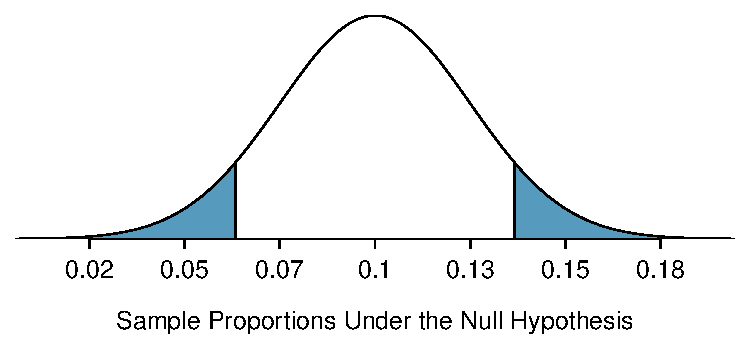
\includegraphics[width=0.7\textwidth]{ch_foundations_for_inf/figures/MedicalConsultant/MedConsNullNormal}
\caption{The shaded area represents the p-value. We observed $\hat{p} = 0.063$, so any observations smaller than this are at least as extreme relative to the null value, $p_0 = 0.1$, and so the lower tail is shaded. However, since this is a two-sided test, values above 0.137 are also at least as extreme as 0.063 (relative to 0.1), and so they also contribute to the p-value. The tail areas together total of about 0.1754 when calculated using a simulation technique in Section~\ref{calcPValueUsingSimulationSubSection}.}
\label{MedConsNullNormal}
\end{figure}

\begin{figure}[ht]
\centering
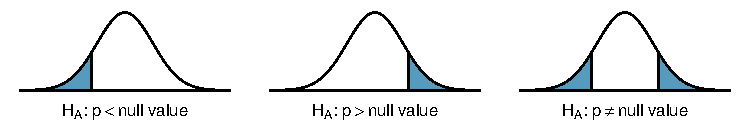
\includegraphics[width=\textwidth]{ch_foundations_for_inf/figures/sidedness/sidedness_example_figures}
\caption{When the alternative hypothesis takes the form $p <$ null value, the p-value is represented by the lower tail. When it takes the form $p >$ null value, the p-value is represented by the upper tail. When using $p \neq$ null value, then the p-value is represented by both tails.}
\label{sidedness_example_figures}
\end{figure}


\begin{onebox}{Finding and interpreting the p-value}
We find and interpret the \term{p-value}\index{hypothesis testing!p-value|textbf} according to the nature of the alternative hypothesis.\vspace{-1mm}
\begin{description}
\setlength{\itemsep}{0mm}

\item[$H_A$: parameter $>$ null value.] The p-value corresponds to the area in the \emph{upper} tail and is probability of getting a test statistic larger than the observed test statistic if the null hypothesis is true and the probability model is accurate.  

\item[$H_A$: parameter $<$ null value.] The p-value corresponds to the area in the \emph{lower} tail and is the probability of observing a test statistic smaller than the observed test statistic if the null hypothesis is true and the probability model is accurate. 

\item[$H_A$: parameter $\ne$ null value.] The p-value corresponds to the area in \emph{both} tails and is the probability of observing a test statistic larger in magnitude than the observed test statistic if the null hypothesis is true and the probability model is accurate. 

\item[] More generally, we can say that the p-value is the probability of getting a test statistic as extreme or more extreme than the observed test statistic in the direction of $H_A$ if the null hypothesis is true and the probability model is accurate.

\end{description}\end{onebox}

When working with proportions, we can also say that the p-value is the probability of getting a sample proportion as far from or farther from the null proportion in the direction of $H_A$ if the null hypothesis is true and the normal model holds.

When the p-value is small, i.e. less than a previously set threshold, we say the results are \term{statistically significant}. This means the data provide such strong evidence against $H_0$ that we reject the null hypothesis in favor of the alternative hypothesis. The threshold is called the \term{significance level}\index{hypothesis testing!significance level}\index{significance level} and is represented by $\alpha$ (the Greek letter \emph{alpha}\label{alphadiscussion}).  The significance level is typically set to $\alpha = 0.05$, but can vary depending on the field or the application. %Using a significance level of $\alpha = 0.05$ in the discrimination study, we can say that the data did not provide statistically significant evidence against the null hypothesis, because the p-value of 0.1754 was larger than the $\alpha$ of 0.05.

\begin{onebox}{Statistical significance}
If the p-value is less than the significance level $\alpha$ (usually 0.05), we say that the result is \term{statistically significant}\index{hypothesis testing!statistically significant|textbf}. We reject $H_0$, and we have strong evidence favoring~$H_A$. \\[2mm]
If the p-value is greater than the significance level $\alpha$, we say that the result is not statistically significant. We do not reject $H_0$, and we do not have strong evidence for $H_A$.\end{onebox}

Recall that the null claim is the claim of no difference. If we reject $H_0$, we are asserting that there is a real difference. If we do not reject $H_0$, we are saying that the null claim is reasonable, but we are not saying that the null claim has been proven.

\begin{exercisewrap}
\begin{nexercise} \label{plainLanguageExplanationOfHTConclusionForLiverDonorSurgicalConsultant}
Because the p-value is 0.1754, which is larger than the significance level 0.05, we do not reject the null hypothesis. Explain what this means in the context of the problem using plain language.\footnotemark
\end{nexercise}
\end{exercisewrap}
\footnotetext{The data do not provide evidence that the consultant's complication rate is significantly lower or higher than the US complication rate of 10\%.}

\D{\newpage}

\begin{examplewrap}
\begin{nexample}{In the previous exercise, we did not reject $H_0$. This means that we did not disprove the null claim. Is this equivalent to proving the null claim is~true?}
No. We did not prove that the consultant's complication rate is \emph{exactly} equal to 10\%. Recall that the test of hypothesis starts by \emph{assuming the null claim is true}. That~is, the test proceeds as an argument by contradiction. \emph{If the null claim is true}, there is a 0.1754 chance of seeing sample data as divergent from 10\% as we saw in our sample. Because 0.1754 is large, it is within the realm of chance error, and we cannot say the null hypothesis is unreasonable.\footnotemark
\end{nexample}
\end{examplewrap}
\footnotetext{The p-value is a conditional probability. It is P(getting data at least as divergent from the null value as we observed $|$ $H_0$ is true). It is NOT P( $H_0$ is true $|$ we got data this divergent from the null value).}


\begin{onebox}{Double negatives can sometimes be used in statistics}
In many statistical explanations, we use double negatives. For instance, we might say that the null hypothesis is \emph{not implausible} or we \emph{failed to reject} the null hypothesis. Double negatives are used to communicate that while we are not rejecting a position, we are also not saying that we know it to be true.\end{onebox}

\begin{examplewrap}
\begin{nexample}{Does the conclusion in Guided Practice~\ref{plainLanguageExplanationOfHTConclusionForLiverDonorSurgicalConsultant} ensure that there is no real association between the surgical consultant's work and the risk of complications? Explain.}
No. It is possible that the consultant's work is associated with a lower or higher risk of complications.
If this was the case, the sample may have been too small
to reliable detect this effect.
\index{data!medical consultant|)}
\end{nexample}
\end{examplewrap}

%The 2-in-100 chance is what we call a \term{p-value}, which is a probability quantifying the strength of the evidence against the null hypothesis and in favor of the alternative. %Formally the p-value is a conditional probability, which is basically\footnote{Want to learn more probability? Check out~Appendix~\ref{probability}.}


%\begin{onebox}{Significance level}
%If the null hypothesis is true, the significance level $\alpha$ defines the probability that we will make a Type~I Error.}
%\end{termBox}

\begin{examplewrap}
\begin{nexample}{An experiment was conducted where study participants were randomly divided into two groups. Both were given the opportunity to purchase a DVD, but one half was reminded that the money, if not spent on the DVD, could be used for other purchases in the future, while the other half was not. The half that was reminded that the money could be used on other purchases was 20\% less likely to continue with a DVD purchase. We determined that such a large difference would only occur about 1-in-150 times if the reminder actually had no influence on student decision-making. What is the p-value in this study? Was the result statistically significant?}
The p-value was 0.006 (about 1/150). Since the p-value is less than 0.05, the data provide statistically significant evidence that US college students were actually influenced by the reminder.
\end{nexample}
\end{examplewrap}

\begin{onebox}{What's so special about 0.05?}
We often use a threshold of 0.05 to determine whether a result is statistically significant. But why 0.05? Maybe we should use a bigger number, or maybe a smaller number. If you're a little puzzled, that probably means you're reading with a critical eye -- good job! We've made a video to help clarify \emph{why 0.05}:
\begin{center}
\oiRedirect{textbook-why05}{www.openintro.org/why05}
\end{center}
Sometimes it's a good idea to deviate from the standard. We'll discuss when to choose a threshold different than 0.05 in Section~\ref{significanceLevel}.\vspace{0.5mm}\end{onebox}

Statistical inference is the practice of making decisions and conclusions from data in the context of uncertainty. Just as a confidence interval may occasionally fail to capture the true value of the parameter, a test of hypothesis may occasionally lead us to an incorrect conclusion. While a given data set may not always lead us to a correct conclusion, statistical inference gives us tools to control and evaluate how often these errors occur.


\D{\newpage}

%%
\subsection{Calculating the p-value by simulation (special topic)}
\label{calcPValueUsingSimulationSubSection}

When conditions for the applying a normal model are met, we use a normal model to find the p-value of a test of hypothesis. In the complication rate example, the distribution is not normal. It is, however, \emph{binomial}, because we are interested in how many out of 142 patients will have complications.

We could calculate the p-value of this test using binomial probabilities. A more general approach, though, for calculating p-values when a normal model does not apply is to use what is known as \term{simulation}. While performing this procedure is outside of the scope of the course, we provide an example here in order to better understand the concept of a p-value.

We simulate 142 new patients to see what result might happen if the complication rate really is 0.10. To do this, we could use a deck of cards. Take one red card, nine black cards, and mix them up. If the cards are well-shuffled, drawing the top card is one way of simulating the chance a patient has a complication if the true rate is 0.10: if the card is red, we say the patient had a complication, and if it is black then we say they did not have a complication. If we repeat this process 142 times and compute the proportion of simulated patients with complications, $\hat{p}_{sim}$, then this simulated proportion is exactly a draw from the null distribution.

There were 12 simulated cases with a complication and 130 simulated cases without a complication: $\hat{p}_{sim} = 12 / 142 = 0.085$.

One simulation isn't enough to get a sense of the null distribution, so we repeated the simulation 10,000 times using a~computer. Figure~\ref{MedConsNullSim} shows the null distribution from these 10,000 simulations. The simulated proportions that are less than or equal to $\hat{p}=0.063$ are shaded. There were 0.0877 simulated sample proportions with $\hat{p}_{sim} \leq 0.063$, which represents a fraction 0.0877 of our simulations:
\begin{align*}
\text{left tail }
	= \frac{\text{Number of observed simulations with }\hat{p}_{sim}\leq\text{ 0.063}}{10000}
	= \frac{877}{10000} = 0.0877
\end{align*}
However, this is not our p-value! Remember that we are conducting a two-sided test, so we should double the one-tail area to get the p-value:\footnote{This doubling approach is preferred even when the distribution isn't symmetric, as in this case.}
\begin{align*}
\text{p-value} = 2 \times \text{left tail} = 2 \times 0.0877 = 0.1754
\end{align*}

\begin{figure}[ht]
\centering
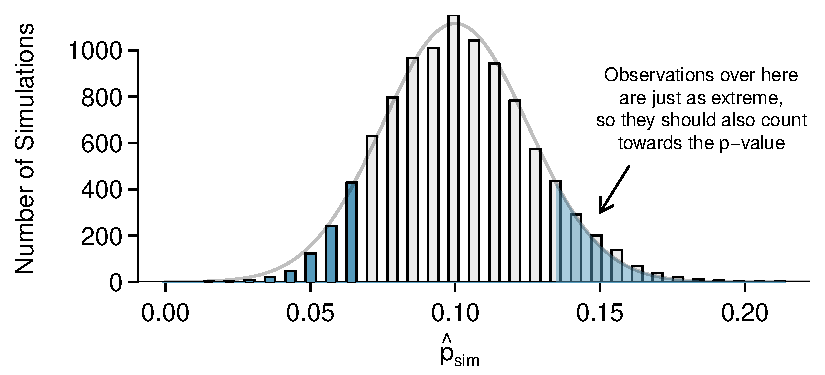
\includegraphics[width=0.8\textwidth]{ch_foundations_for_inf/figures/MedicalConsultant/MedConsNullSim}
\caption{The null distribution for $\hat{p}$, created from 10,000 simulated studies. The left tail contains 8.77\% of the simulations. For a two-sided test, we double the tail area to get the p-value. This doubling accounts for the observations we might have observed in the upper tail, which are also at least as extreme (relative to 0.10) as what we observed, $\hat{p} = 0.063$.}
\label{MedConsNullSim}
\end{figure}


\D{\newpage}

%%
\subsection{Hypothesis testing: a five step process}
Use a hypothesis test to \emph{test} $H_0$ versus $H_A$ at a particular \emph{signficance level}, $\alpha$.

\begin{onebox}{(AP exam tip) When carrying out a hypothesis test procedure, follow these five steps:}
\begin{itemize}
\setlength{\itemsep}{0mm}
\item \inferencestep{Identify}  Identify the hypotheses and the significance level.
\item  \inferencestep{Choose}  Choose the appropriate test procedure and identify it by name.
\item  \inferencestep{Check}  Check that the conditions for the test procedure are met. 
\item \inferencestep{Calculate} Calculate the test statistic and the p-value.  
\begin{align*}
\text{test statistic} = \frac{\text{point estimate } - \text{ null value}}{SE\ \text{of estimate}}
\end{align*}
\item \inferencestep{Conclude} Compare the p-value to the significance level to determine whether to reject $H_0$ or not reject $H_0$.  Draw a conclusion in the context of $H_A$.  
\end{itemize}\end{onebox}

%%
\subsection{Decision errors}
\index{hypothesis testing!decision errors|(}
The hypothesis testing framework is a very general tool, and we often use it without a second thought. If a person makes a somewhat unbelievable claim, we are initially skeptical. However, if there is sufficient evidence that supports the claim, we set aside our skepticism. The hallmarks of hypothesis testing are also found in the US court system. 

\begin{examplewrap}
\begin{nexample}{A US court considers two possible claims about a defendant: she is either innocent or guilty. If we set these claims up in a hypothesis framework, which would be the null hypothesis and which the alternative?}\label{hypTestCourtExample}
The jury considers whether the evidence is so convincing (strong) that there is evidence beyond a reasonable doubt of the person's guilt. That is, the starting assumption (null hypothesis) is that the person is innocent until evidence is presented that convinces the jury that the person is guilty (alternative hypothesis). In statistics, our evidence comes in the form of data, and we use the significance level to decide what is beyond a reasonable doubt.
\end{nexample}
\end{examplewrap}

Jurors examine the evidence to see whether it convincingly shows a defendant is guilty. Notice that a jury finds a defendant either guilty or not guilty. They either reject the null claim or they do not reject the null claim. They never prove the null claim, that is, they never find the defendant innocent. If a jury finds a defendant \emph{not guilty}, this does not necessarily mean the jury is confident in the person's innocence. They are simply not convinced of the alternative that the person is guilty.

This is also the case with hypothesis testing: \emph{even if we fail to reject the null hypothesis, we typically do not accept the null hypothesis as truth}. Failing to find strong evidence for the alternative hypothesis is not equivalent to providing evidence that the null hypothesis is true.


Hypothesis tests are not flawless. Just think of the court system: innocent people are sometimes wrongly convicted and the guilty sometimes walk free. Similarly, data can point to the wrong conclusion. However, what distinguishes statistical hypothesis tests from a court system is that our framework allows us to quantify and control how often the data lead us to the incorrect conclusion.

There are two competing hypotheses: the null and the alternative. In a hypothesis test, we make a statement about which one might be true, but we might choose incorrectly. There are four possible scenarios in a hypothesis test, which are summarized in Figure~\ref{fourHTScenarios}.

\begin{figure}[ht]
\centering
\begin{tabular}{l l c c c}
& & \multicolumn{2}{c}{\textbf{Test conclusion}} \\
  \cline{3-4}
\vspace{-3.7mm} \\
& & do not reject $H_0$ &  reject $H_0$ in favor of $H_A$ &
\ \hspace{7mm} \  \\
  \cline{2-4}
\vspace{-3.7mm} \\
& $H_0$ true & correct conclusion &  Type~I Error \\
\raisebox{1.5ex}{\textbf{Truth}} & $H_A$ true & Type~II Error & correct conclusion \\
  \cline{2-4}
\end{tabular}
\caption{Four different scenarios for hypothesis tests.}
\label{fourHTScenarios}
\end{figure}

\begin{onebox}{Type~I and Type~II Errors}
A \term{Type~I Error} is rejecting $H_0$ when $H_0$ is actually true. When we reject the null hypothesis, it is possible that we make a Type~I Error. \\[2mm]
A \term{Type~II Error} is failing to reject $H_0$ when $H_A$ is actually true. When we dod not reject the null hypothesis, it is possible that we make a Type~II Error.\end{onebox}



\begin{examplewrap}
\begin{nexample}{In a US court, the defendant is either innocent ($H_0$) or guilty ($H_A$). What does a Type~I Error represent in this context? What does a Type~II Error represent? Figure~\ref{fourHTScenarios} may be useful.}
If the court makes a Type~I Error, this means the defendant is innocent ($H_0$ true) but wrongly convicted. A~Type~II Error means the court failed to reject $H_0$ (i.e. failed to convict the person) when they were in fact guilty ($H_A$ true).
\end{nexample}
\end{examplewrap}

\begin{examplewrap}
\begin{nexample}{How could we reduce the Type~I Error rate in US courts? What influence would this have on the Type~II Error rate?}
To lower the Type~I Error rate, we might raise our standard for conviction from ``beyond a reasonable doubt'' to ``beyond a conceivable doubt'' so fewer people would be wrongly convicted. However, this would also make it more difficult to convict the people who are actually guilty, so we would make more Type~II Errors.
\end{nexample}
\end{examplewrap}

\begin{exercisewrap}
\begin{nexercise} \label{howToReduceType2ErrorsInUSCourts}
How could we reduce the Type~II Error rate in US courts? What influence would this have on the Type~I Error rate?\footnotemark
\end{nexercise}
\end{exercisewrap}
\footnotetext{To lower the Type~II Error rate, we want to convict more guilty people. We could lower the standards for conviction from ``beyond a reasonable doubt'' to ``beyond a little doubt''. Lowering the bar for guilt will also result in more wrongful convictions, raising the Type~I Error rate.}

\begin{exercisewrap}
\begin{nexercise}
A group of women bring a class action lawsuit that claims discrimination in promotion rates. What would a Type~I Error represent in this context?\footnotemark
\end{nexercise}
\end{exercisewrap}
\footnotetext{We must first identify which is the null hypothesis and which is the alternative. The alternative hypothesis is the one that bears the burden of proof, so the null hypothesis is that there was no discrimination and the alternative hypothesis is that there was discrimination. Making a Type~I Error in this context would mean that in fact there was no discrimination, even though we concluded that women were discriminated against. Notice that this does \emph{not} necessarily mean something was wrong with the data or that we made a computational mistake. Sometimes data simply point us to the wrong conclusion, which is why scientific studies are often repeated to check initial findings.}

\index{hypothesis testing!decision errors|)}

These examples provide an important lesson: if we reduce how often we make one type of error, we generally make more of the other type.

%Hypothesis testing is built around rejecting or failing to reject the null hypothesis. That is, we do not reject $H_0$ unless the data provide strong evidence against it. But what precisely does \emph{strong evidence} mean? As a general rule of thumb, for those cases where the null hypothesis is actually true, we do not want to incorrectly reject $H_0$ more than 5\% of the time. This corresponds to our default significance level of $\alpha = 0.05$, which we use as a comparison with the p-value. In the next section, we discuss the appropriateness of different significance levels.


\D{\newpage}

%%
\subsection{Choosing a significance level}
\label{significanceLevel}

\index{hypothesis testing!significance level|(}
\index{significance level|(}

If $H_0$ is true, what is the probability that we will incorrectly reject it? In hypothesis testing, we perform calculations under the premise that $H_0$ is true, and we reject $H_0$ if the p-value is smaller than the significance level $\alpha$. That is, $\alpha$ \emph{is} the probability of making a Type~I Error. The choice of what to make $\alpha$ is not arbitrary. It depends on the gravity of the consequences of a Type~I Error.

\begin{onebox}{Relationship between Type~I and Type~II Errors}
The probability of a Type~I Error is called $\alpha$ and corresponds to the significance level of a test. The probability of a Type~II Error is called $\beta$. As we make $\alpha$ smaller, $\beta$ typically gets larger, and vice versa.\end{onebox}

\begin{examplewrap}
\begin{nexample}{If making a Type~I Error is especially dangerous or especially costly, should we choose a smaller significance level or a higher significance level?}
Under this scenario, we want to be very cautious about rejecting the null hypothesis, so we demand very strong evidence before we are willing to reject the null hypothesis. Therefore, we want a smaller significance level, maybe $\alpha = 0.01$.
\end{nexample}
\end{examplewrap}

\begin{examplewrap}
\begin{nexample}{If making a Type~II Error is especially dangerous or especially costly, should we choose a smaller significance level or a higher significance level?}
We should choose a higher significance level (e.g. 0.10). Here we want to be cautious about failing to reject $H_0$ when the null is actually false.
\end{nexample}
\end{examplewrap}

\begin{onebox}{Significance levels should reflect consequences of errors}
The significance level selected for a test should reflect the real-world consequences associated with making a Type~I or Type~II Error. If a Type~I Error is very dangerous, make $\alpha$ smaller.\end{onebox}

\index{hypothesis testing!significance level|)}
\index{significance level|)}


%%
\subsection{Statistical power of a hypothesis test}

When the alternative hypothesis is true, the probability of \underline{not} making a Type~II Error is called \term{power}. It is common for researchers to perform a \hiddenterm{power analysis} to ensure their study collects enough data to detect the effects they anticipate finding. As you might imagine, if the effect they care about is small or subtle, then if the effect is real, the researchers will need to collect a large sample size in order to have a good chance of detecting the effect. However, if they are interested in large effect, they need not collect as much data.

The Type~II Error rate $\beta$ and the magnitude of the error for a point estimate are controlled by the sample size. As the sample size $n$ goes up, the Type~II Error rate goes down, and power goes up. Real differences from the null value, even large ones, may be difficult to detect with small samples. However, if we take a very large sample, we might find a statistically significant difference but the size of the difference might be so small that it is of no practical value.

\index{hypothesis testing|)}


\D{\newpage}

%%
\subsection*{Section summary}


\begin{itemize}
\item A \term{hypothesis test} is a statistical technique used to evaluate competing claims based on data.  

\item The competing claims are called \term{hypotheses} and are often about population parameters (e.g. $\mu$ and $p$); they are never about sample statistics.  \vspace{-1mm}
\begin{itemize}
\item The \term{null hypothesis} is abbreviated $H_0$. It represents a skeptical perspective or a perspective of no difference or \emph{no change}.
\item The \term{alternative hypothesis} is abbreviated $H_A$. It represents a new perspective or a perspective of a real difference or change.  Because the alternative hypothesis is the stronger claim, it bears the burden of proof.  
\end{itemize}

\item The \term{logic of a hypothesis test}\index{hypothesis test!logic of}:  In a hypothesis test, we begin by \textit{assuming that the null hypothesis is true}.  Then, we calculate how unlikely it would be to get a sample value as extreme as we actually got in our sample, assuming that the null value is correct.  If this likelihood is too small, it casts doubt on the null hypothesis and provides evidence for the alternative hypothesis.

\item We set a \term{significance level}, denoted $\alpha$, which represents the threshold below which we will reject the null hypothesis.  The most common significance level is $\alpha = 0.05$.  If we require more evidence to reject the null hypothesis, we use a smaller $\alpha$.

\item After verifying that the relevant \term{conditions are met}, we can calculate the test statistic.  The \term{test statistic} tells us \textit{how many} standard errors the point estimate (sample value) is from the null value (i.e. the value hypothesized for the parameter in the null hypothesis).  When investigating a single mean or proportion or a difference of means or proportions, the test statistic is calculated as: $\frac{\text{point estimate } -\text{ null value}}{SE \text{ of estimate}}$.

\item After the test statistic, we calculate the p-value.  We find and interpret the p-value according to the nature of the alternative hypothesis.  The three possibilities are:\vspace{-1mm}
\begin{itemize}
\item[] $H_A$: parameter $>$ null value. \quad\parbox[t]{3.84in}{The p-value corresponds to the area in the \emph{upper tail}.  }
\item[] $H_A$: parameter $<$ null value. \quad\parbox[t]{3.84in}{The p-value corresponds to the area in the \emph{lower tail}.  }
\item[] $H_A$: parameter $\ne$ null value. \quad\parbox[t]{3.84in}{The p-value corresponds to the area in \emph{both tails}.  }
\end{itemize}
The \term{p-value} is the probability of getting a test statistic as extreme or more extreme than the observed test statistic in the direction of $H_A$ if the null hypothesis is true and the probability model is accurate.

\item The conclusion or decision of a hypothesis test is based on whether the p-value is smaller or larger than the preset significance level $\alpha$. \vspace{-1mm}
\begin{itemize}
\item When the  p-value $< \alpha$, we say the results are \term{statistically significant} at the $\alpha$ level and we have evidence of a real difference or change.  The observed difference is beyond what would have been expected from chance variation alone.  This leads us to reject $H_0$ and gives us evidence for $H_A$.
\item When the  p-value $> \alpha$, we say the results are not statistically significant at the $\alpha$ level and we do not have evidence of a real difference or change.  The observed difference was within the realm of expected chance variation.  This leads us to not reject $H_0$ and does not give us evidence for $H_A$.
\end{itemize}

\D{\newpage}

\item AP exam tip:  A full hypothesis test includes the following steps.\vspace{-1mm}
\begin{enumerate}
\setlength{\itemsep}{0mm}
\item \inferencestep{Identify}  Identify the hypotheses and the significance level.
\item  \inferencestep{Choose}  Choose the appropriate test procedure and identify it by name.
\item  \inferencestep{Check}  Check that the conditions for the test procedure are met. 
\item \inferencestep{Calculate} Calculate the test statistic and the p-value.  
\begin{align*}
\text{test statistic} = \frac{\text{point estimate } - \text{ null value}}{SE\ \text{of estimate}}
\end{align*}
\item \inferencestep{Conclude} Compare the p-value to the significance level to determine whether to reject $H_0$ or not reject $H_0$.  Draw a conclusion in the context of $H_A$.\end{enumerate}

\item \termsub{Decision errors}{decision errors}.  In a hypothesis test, there are two types of decision errors that could be made.  These are called Type~I and Type~II Errors. \vspace{-1mm}
\begin{itemize}
\item A \term{Type~I Error} is rejecting $H_0$, when $H_0$ is actually true.  We commit a Type~I Error if we call a result significant when there is \emph{no} real difference or effect.  P(Type I~error) = $\alpha$.
\item A \term{Type~II Error} is not rejecting $H_0$, when $H_A$ is actually true.  We commit a Type~II Error if we call a result not significant when there \emph{is} a real difference or effect.  P(Type II~error) = $\beta$.
\item The probability of a Type~I Error ($\alpha$) and a Type~II Error ($\beta$) are \emph{inversely related}. Decreasing $\alpha$ makes $\beta$ larger; increasing $\alpha$ makes $\beta$ smaller.  
\item Once a decision is made, only one of the two types of errors is possible.  If the test rejects $H_0$, for example, only a Type~I Error is possible.
\end{itemize}
\item The power of a test.
\begin{itemize}\vspace{-1mm}
\setlength{\itemsep}{0mm}
\item When a particular $H_A$ is true, the probability of not making a Type~II Error is called \term{power}.  Power $= 1 - \beta$.  
\item The power of a test is the probability of detecting an effect of a particular size when it is present.
\item Increasing the significance level decreases the probability of a Type~II Error and increases power.  $\alpha \uparrow, \beta \downarrow, \text{power} \uparrow$.  
\item For a fixed $\alpha$, increasing the sample size $n$ makes it easier to detect an effect and therefore decreases the probability of a Type~II Error and increases power.   $n \uparrow, \beta \downarrow, \text{power} \uparrow$.


\end{itemize}
\end{itemize}


%%%%%%Section exercises
{\exercisesheader{}

% 13 - identify_hypotheses_prop_and_mean_1

\eoce{\qt{Identify hypotheses, Part I\label{
}}
Write the null and alternative hypotheses in words and then symbols
for each of the following  situations.
\begin{parts}
\item
    A tutoring company would like to understand if most
    students tend to improve their grades (or not) after
    they use their services.
    They sample 200 of the students who used their service
    in the past year and ask them if their grades have
    improved or declined from the previous year.
\item
    Employers at a firm are worried about the effect of March Madness,
    a basketball championship held each spring in the US, on employee
    productivity.
    They estimate that on a regular business day employees spend on
    average 15 minutes of company time checking personal email,
    making personal phone calls, etc.
    They also collect data on how much company time employees spend
    on such non-business activities during March Madness.
    They want to determine if these data provide convincing evidence
    that employee productivity changed during March Madness.
\end{parts}
}{}

% 14 - identify_hypotheses_prop_and_mean_2

\eoce{\qt{Identify hypotheses, Part II\label{identify_hypotheses_prop_and_mean_2}} 
Write the null and alternative hypotheses in words and using symbols 
for each of the following situations.
\begin{parts}
\item
    Since 2008, chain restaurants in California have been required
    to display calorie counts of each menu item. Prior to menus
    displaying calorie counts, the average calorie intake of diners
    at a restaurant was 1100 calories.
    After calorie counts started to be displayed on menus,
    a nutritionist collected data on the number of calories consumed
    at this restaurant from a random sample of diners.
    Do these data provide convincing evidence of a difference in the
    average calorie intake of a diners at this restaurant?
\item
    The state of Wisconsin would like to understand
    the fraction of its adult residents that consumed alcohol
    in the last year,
    specifically if the rate is different from the
    national rate of 70\%.
    To help them answer this question, they conduct
    a random sample of 852 residents and ask them
    about their alcohol consumption.
\end{parts}
}{}

% 15 - online_communication_prop_ht_errors

\eoce{\qt{Online communication\label{online_communication_prop_ht_errors}}
A study suggests that 60\% of college student spend
10~or more hours per week communicating with others online.
You believe that this is incorrect and decide to collect your 
own sample for a hypothesis test.
You randomly sample 160 students from your dorm
and find that 70\% spent 10~or more hours a week
communicating with others online.
A~friend of yours, who offers to help you with
the hypothesis test, comes up with the following
set of hypotheses.
Indicate any errors you see.
\begin{align*}
H_0&: \hat{p} < 0.6 \\
H_A&: \hat{p} > 0.7
\end{align*}
}{}

% 16 - married_at_25_prop_ht_errors

\eoce{\qt{Married at 25\label{married_at_25_prop_ht_errors}}
A study suggests that the 25\% of 25 year olds have
gotten married.
You believe that this is incorrect and decide to collect
your own sample for a hypothesis test.
From a random sample of 25 year olds in census data
with size 776,
you find that 24\% of them are married.
A friend of yours offers to help you with setting
up the hypothesis test and comes up with the following
hypotheses.
Indicate any errors you see.
\begin{align*}
H_0&: \hat{p} = 0.24 \\
H_A&: \hat{p} \neq 0.24
\end{align*}
}{}

% 17 - cyberbullying_prop_ci_ht

\eoce{\qt{Cyberbullying rates\label{cyberbullying_prop_ci_ht}}
Teens were surveyed about cyberbullying, and
54\% to 64\% reported experiencing cyberbullying
(95\% confidence interval).\footfullcite{pew_cyber_bully_2018}
Answer the following questions based on this interval.
\begin{parts}
\item 
    A newspaper claims that a majority of teens
    have experienced cyberbullying.
    Is this claim supported by the confidence interval?
    Explain your reasoning.
\item\label{cyberbullying_prop_ci_ht_researcher}
    A researcher conjectured that 70\% of teens have
    experienced cyberbullying.
    Is this claim supported by the confidence interval?
    Explain your reasoning.
\item
    Without actually calculating the interval, determine
    if the claim of the researcher from
    part~(\ref{cyberbullying_prop_ci_ht_researcher})
    would be supported based on a 90\% confidence interval?
\end{parts}
}{}

% 18 - er_wait_ci_ht_prop_ok

\eoce{\qt{Waiting at an ER, Part II\label{er_wait_ci_ht_prop_ok}}
Exercise~\ref{er_wait_intro_prop_ok} 
provides a 95\% confidence interval for the mean waiting
time at an emergency room (ER) of (128 minutes, 147 minutes).
Answer the following questions based on this interval.
\begin{parts}
\item
    A local newspaper claims that the average waiting time
    at this ER exceeds 3 hours.
    Is this claim supported by the confidence interval?
    Explain your reasoning.
\item\label{er_wait_ci_ht_prop_ok_dean}
    The Dean of Medicine at this hospital claims the
    average wait time is 2.2 hours.
    Is this claim supported by the confidence interval?
    Explain your reasoning.
\item
    Without actually calculating the interval,
    determine if the claim of the Dean from
    part~(\ref{er_wait_ci_ht_prop_ok_dean})
    would be supported based on a 99\% confidence interval?
\end{parts}
}{}

% 19 - minimum_wage_prop_1

\eoce{\qt{Minimum wage, Part I\label{minimum_wage_prop_1}}
Do a majority of US adults believe raising
the minimum wage will help the economy,
or is there a majority who do not believe this?
A~Rasmussen Reports survey of 1,000 US adults found
that 42\% believe it will help the
economy.\footfullcite{webpage:rasmussen-2019-raise-minimum-wage}
Conduct an appropriate hypothesis test to help
answer the research question.
}{}

% 20 - univ_students_enough_sleep

\eoce{\qt{Getting enough sleep\label{univ_students_enough_sleep}}
400 students were randomly sampled from a large university,
and 289 said they did not get enough sleep.
Conduct a hypothesis test to check whether this
represents a statistically significant difference
from 50\%, and use a significance level of 0.01.
}{}

% 21 - backwards_prop_1

\eoce{\qt{Working backwards, Part I\label{backwards_prop_1}}
You are given the following hypotheses:
\begin{align*}
H_0&: p = 0.3 \\
H_A&: p \ne 0.3
\end{align*}
We know the sample size is 90.
For what sample proportion would the p-value be equal to 0.05?
Assume that all conditions  necessary for inference are satisfied.
}{}

% 22 - backwards_prop_2

\eoce{\qt{Working backwards, Part II\label{backwards_prop_2}}
You are given the following hypotheses:
\begin{align*}
H_0&: p = 0.9 \\
H_A&: p \ne 0.9
\end{align*}
We know that the sample size is 1,429.
For what sample proportion would the p-value be equal to 0.01?
Assume that all conditions necessary for inference are satisfied.
}{}

% 23 - errors_fibromyalgia

\eoce{\qt{Testing for Fibromyalgia\label{errors_fibromyalgia}} A patient named Diana 
was diagnosed with Fibromyalgia, a long-term syndrome of body pain, and was 
prescribed anti-depressants. Being the skeptic that she is, Diana didn't 
initially believe that anti-depressants would help her symptoms. However after 
a couple months of being on the medication she decides that the 
anti-depressants are working, because she feels like her symptoms are in fact 
getting better.
\begin{parts}
\item Write the hypotheses in words for Diana's skeptical position when she 
started taking the anti-depressants.
\item What is a Type~1 Error in this context?
\item What is a Type~2 Error in this context?
\end{parts}
}{}

% 24 - prop_which_higher_found_inf

\eoce{\qtq{Which is higher\label{prop_which_higher_found_inf}}
In each part below, there is a value of interest and two
scenarios (I and II).
For each part, report if the value of interest is larger
under scenario I, scenario II, or whether the value is
equal under the scenarios.
\begin{parts}
\item
     The standard error of $\hat{p}$ when
     (I)~$n = 125$ or (II)~$n = 500$.
\item
    The margin of error of a confidence interval
    when the confidence level is
    (I)~90\% or (II)~80\%.
\item
    The p-value for a Z-statistic of 2.5 calculated
    based on a (I)~sample with $n = 500$ or based on
    a (II)~sample with $n = 1000$.
\item
    The probability of making a Type~2 Error when the
    alternative hypothesis is true and the significance
    level is (I)~0.05 or (II)~0.10.
\end{parts}
}{}
}

%______________________________________
\section{Does it make sense?}
\sectionintro{
\noindent%
It is the responsibility of the data scientist to know when the use of these inference procedures is appropriate and to correctly interpret the results.
In~this section, we look at considerations around the misuse or misinterpretation of these procedures.


%%
\subsection*{Learning objectives}
\begin{enumerate}
\item Understand the two general conditions for when the confidence interval and hypothesis testing procedures apply.  Explain why these conditions are necessary.

\item Distinguish between statistically significant and practically significant.  What role does sample size play here?

\item Recognize that not all statistically significant results correspond to real differences, due to Type~I Errors.  What role does the significance level $\alpha$ play here?
\end{enumerate}
}

%%
\subsection{When to retreat}
\label{whenToRetreat}



Statistical tools rely on conditions. When the conditions are not met, these tools are unreliable and drawing conclusions from them is treacherous. The conditions for these tools typically come in two forms.
\begin{itemize}
\setlength{\itemsep}{0mm}
\item \textbf{The individual observations must be independent.} A random sample from less than 10\% of the population ensures the observations are independent. In experiments, we generally require that subjects are randomized into groups. If independence fails, then advanced techniques must be used, and in some such cases, inference may not be possible.
\item \textbf{Other conditions focus on sample size and skew.} For example, if the sample size is too small, the skew too strong, or extreme outliers are present, then a normal model for the sample mean will fail.
\end{itemize}
Verification of conditions for statistical tools is always necessary. Whenever conditions are not satisfied for a statistical technique, there are three options. The first is to learn new methods that are appropriate for the data. The second route is to consult a data scientist.\footnote{If you work at a university, then there may be campus consulting services to assist you. Alternatively, there are many private consulting firms that are also available for hire.} The third route is to ignore the failure of conditions. This last option effectively invalidates any analysis and may discredit novel and interesting findings.

Finally, we caution that there may be no inference tools helpful when considering data that include unknown biases, such as convenience samples. For this reason, there are books, courses, and researchers devoted to the techniques of sampling and experimental design. See Sections~\ref{overviewOfDataCollectionPrinciples}-\ref{experimentsSection} for basic principles of data collection.


\D{\newpage}

%%
\subsection{Statistical significance versus practical significance}

When the sample size becomes larger, point estimates become more precise and any real differences in the mean and null value become easier to detect and recognize. Even a very small difference would likely be detected if we took a large enough sample. Sometimes researchers will take such large samples that even the slightest difference is detected. While we still say that difference is \term{statistically significant}, it might not be \term{practically significant}.

Statistically significant differences are sometimes so minor that they are not practically relevant. This is especially important to research: if we conduct a study, we want to focus on finding a meaningful result. We don't want to spend lots of money finding results that hold no practical value.

The role of a data scientist in conducting a study often includes planning the size of the study. The data scientist might first consult experts or scientific literature to learn what would be the smallest meaningful difference from the null value. She also would obtain some reasonable estimate for the standard deviation. With these important pieces of information, she would choose a sufficiently large sample size so that the power for the meaningful difference is perhaps 80\% or 90\%. While larger sample sizes may still be used, she might advise against using them in some cases, especially in sensitive areas of research.

\subsection{Statistical significance versus a real difference}

When a result is statistically significant at the $\alpha=0.05$ level, we have evidence that the result is real.
However, when there is no difference or effect, we can expect that 5\% of the time the test conclusion will lead to a Type~I Error and incorrectly reject the null hypothesis.
Therefore we must beware of what is called p-hacking, in which researchers may test many, many hypotheses and then publish the ones that come out statistically significant.
As we noted, we can expect 5\% of the results to be significant when the null hypothesis is true and there really is no difference or effect.\footnote{
The problem is even greater than p-hacking.  In what has been called the ``reproducibility crisis", researchers have failed to reproduce a large proportion of results that were found significant and were published in scientific journals.
This problem highlights the importance of research that
reproduces earlier work rather than taking the word of
a single study.

Also keep in mind that the probability that a difference will be found to be significant given that there is no real difference is not the same as the probability that a difference is not real, given that it was found significant.
Depending upon the veracity of the hypotheses tested, the latter can be upwards of 80\%, leading some to assert that ``most published research is false". \\
\oiRedirect{textbook-trouble-at-the-lab}{\url{https://www.economist.com/briefing/2013/10/18/trouble-at-the-lab}}
}


\D{\newpage}

%%
\subsection*{Section summary}
\noindent The inference procedures in this book require \emph{two conditions} to be met.
\begin{itemize}
\item The first is that some type of \term{random sampling} or \term{random assignment} must be involved.  If this is not the case, the point statistic may be biased and may not follow the intended distribution.  Moreover, without a random sample or random assignment, there is no way to accurately measure the standard error.  (When sampling without replacement, the sample size should be less than 10\% of the population size in order for the standard error formula to apply.  In sample surveys, this condition is generally met.)
\item The second condition focuses on \term{sample size} and \term{skew} to determine whether the point estimate follows the intended distribution.  
\end{itemize}
Understanding what the term \term{statistically significant} does and does not mean.
\begin{itemize}
\item \emph{A small percent of the time ($\alpha$), a significant result will not be a real result.} If many tests are run, a small percent of them will produce significant results due to chance alone.\footnote{Similarly, if many confidence intervals are constructed, a small percent (100 - C\%) of them will fail to capture a true value due to chance alone.  A value outside the confidence interval is not an \emph{impossible} value.}

\item \emph{With a very large sample, a significant result may point to a result that is real but unimportant}. With a larger sample, the power of a test increases and it becomes easier to detect a small difference.  If an extremely large sample is used, the result may be statistically significant, but not be \emph{practically significant}.  That is, the difference detected may be so small as to be unimportant or meaningless.  
\end{itemize}


\newpage
%______________________________________________
\reviewchapterheader{}

\noindent Statistical inference is the practice of making decisions from data in the context of uncertainty.  In this chapter, we introduced two frameworks for inference:  \termsub{confidence intervals}{confidence interval} and \termsub{hypothesis tests}{hypothesis test}.   
\begin{itemize}
\item Confidence intervals are used for \textit{estimating} unknown population parameters by providing an \textit{interval of reasonable values} for the unknown parameter with a certain level of confidence.
\item Hypothesis tests are used to assess how reasonable a \textit{particular} value is for an unknown population parameter by providing \textit{degrees of evidence} against that value.
\item The results of confidence intervals and hypothesis tests are, generally speaking, \textit{consistent}.\footnote{In the context of proportions there will be a small range of cases where this is not true.  This is because when working with proportions, the $SE$ used for confidence intervals and the $SE$ used for tests are slightly different, as we will see in the next chapter.}  That is:\vspace{-1mm}
\begin{itemize}
\item Values that fall \textit{inside} a 95\% confidence interval (implying they are reasonable) will \textit{not be rejected} by a test at the 5\% significance level (implying they are reasonable), and vice-versa.  
\item Values that fall \textit{outside} a 95\% confidence interval (implying they are not reasonable) will \textit{be rejected} by a test at the 5\% significance level (implying they are not reasonable), and vice-versa.
\item When the confidence level and the significance level add up to 100\%, the conclusions of the two procedures are consistent.
\end{itemize}
\item Many values fall inside of a confidence interval and will not be rejected by a hypothesis test. ``Not rejecting $H_0$" is NOT equivalent to \textit{accepting} $H_0$.   When we ``do not reject $H_0$", we are asserting that the null value is \textit{reasonable}, not that the parameter is exactly \emph{equal to} the null value.
\item For a 95\% confidence interval, 95\% is not the probability that the true value lies inside the confidence interval (it either does or it doesn't).  Likewise, for a hypothesis test, $\alpha$ is not the probability that $H_0$ is true (it either is or it isn't).  In both frameworks, the probability is about what would happen in a random sample, not about what is true of the population.  
\item The confidence interval procedures and hypothesis tests described in this book should not be applied unless particular conditions (described in more detail in the following chapters) are met.  If these procedures are applied when the conditions are not met, the results may be unreliable and misleading.  
\end{itemize}
 While a given data set may not always lead us to a correct conclusion, statistical inference gives us tools to \textit{control and evaluate how often errors occur}.


